\documentclass[twoside]{book}

% Packages required by doxygen
\usepackage{fixltx2e}
\usepackage{calc}
\usepackage{doxygen}
\usepackage[export]{adjustbox} % also loads graphicx
\usepackage{graphicx}
\usepackage[utf8]{inputenc}
\usepackage{makeidx}
\usepackage{multicol}
\usepackage{multirow}
\PassOptionsToPackage{warn}{textcomp}
\usepackage{textcomp}
\usepackage[nointegrals]{wasysym}
\usepackage[table]{xcolor}

% Font selection
\usepackage[T1]{fontenc}
\usepackage[scaled=.90]{helvet}
\usepackage{courier}
\usepackage{amssymb}
\usepackage{sectsty}
\renewcommand{\familydefault}{\sfdefault}
\allsectionsfont{%
  \fontseries{bc}\selectfont%
  \color{darkgray}%
}
\renewcommand{\DoxyLabelFont}{%
  \fontseries{bc}\selectfont%
  \color{darkgray}%
}
\newcommand{\+}{\discretionary{\mbox{\scriptsize$\hookleftarrow$}}{}{}}

% Page & text layout
\usepackage{geometry}
\geometry{%
  a4paper,%
  top=2.5cm,%
  bottom=2.5cm,%
  left=2.5cm,%
  right=2.5cm%
}
\tolerance=750
\hfuzz=15pt
\hbadness=750
\setlength{\emergencystretch}{15pt}
\setlength{\parindent}{0cm}
\setlength{\parskip}{0.2cm}
\makeatletter
\renewcommand{\paragraph}{%
  \@startsection{paragraph}{4}{0ex}{-1.0ex}{1.0ex}{%
    \normalfont\normalsize\bfseries\SS@parafont%
  }%
}
\renewcommand{\subparagraph}{%
  \@startsection{subparagraph}{5}{0ex}{-1.0ex}{1.0ex}{%
    \normalfont\normalsize\bfseries\SS@subparafont%
  }%
}
\makeatother

% Headers & footers
\usepackage{fancyhdr}
\pagestyle{fancyplain}
\fancyhead[LE]{\fancyplain{}{\bfseries\thepage}}
\fancyhead[CE]{\fancyplain{}{}}
\fancyhead[RE]{\fancyplain{}{\bfseries\leftmark}}
\fancyhead[LO]{\fancyplain{}{\bfseries\rightmark}}
\fancyhead[CO]{\fancyplain{}{}}
\fancyhead[RO]{\fancyplain{}{\bfseries\thepage}}
\fancyfoot[LE]{\fancyplain{}{}}
\fancyfoot[CE]{\fancyplain{}{}}
\fancyfoot[RE]{\fancyplain{}{\bfseries\scriptsize Generated on Sun Dec 20 2015 23\+:08\+:05 for R\+H\+I\+C\+F\+Detector\+Construction by Doxygen }}
\fancyfoot[LO]{\fancyplain{}{\bfseries\scriptsize Generated on Sun Dec 20 2015 23\+:08\+:05 for R\+H\+I\+C\+F\+Detector\+Construction by Doxygen }}
\fancyfoot[CO]{\fancyplain{}{}}
\fancyfoot[RO]{\fancyplain{}{}}
\renewcommand{\footrulewidth}{0.4pt}
\renewcommand{\chaptermark}[1]{%
  \markboth{#1}{}%
}
\renewcommand{\sectionmark}[1]{%
  \markright{\thesection\ #1}%
}

% Indices & bibliography
\usepackage{natbib}
\usepackage[titles]{tocloft}
\setcounter{tocdepth}{3}
\setcounter{secnumdepth}{5}
\makeindex

% Hyperlinks (required, but should be loaded last)
\usepackage{ifpdf}
\ifpdf
  \usepackage[pdftex,pagebackref=true]{hyperref}
\else
  \usepackage[ps2pdf,pagebackref=true]{hyperref}
\fi
\hypersetup{%
  colorlinks=true,%
  linkcolor=blue,%
  citecolor=blue,%
  unicode%
}

% Custom commands
\newcommand{\clearemptydoublepage}{%
  \newpage{\pagestyle{empty}\cleardoublepage}%
}


%===== C O N T E N T S =====

\begin{document}

% Titlepage & ToC
\hypersetup{pageanchor=false,
             bookmarks=true,
             bookmarksnumbered=true,
             pdfencoding=unicode
            }
\pagenumbering{roman}
\begin{titlepage}
\vspace*{7cm}
\begin{center}%
{\Large R\+H\+I\+C\+F\+Detector\+Construction \\[1ex]\large 1.\+0.\+0 }\\
\vspace*{1cm}
{\large Generated by Doxygen 1.8.10}\\
\vspace*{0.5cm}
{\small Sun Dec 20 2015 23:08:05}\\
\end{center}
\end{titlepage}
\clearemptydoublepage
\tableofcontents
\clearemptydoublepage
\pagenumbering{arabic}
\hypersetup{pageanchor=true}

%--- Begin generated contents ---
\chapter{Hierarchical Index}
\section{Class Hierarchy}
This inheritance list is sorted roughly, but not completely, alphabetically\+:\begin{DoxyCompactList}
\item G4\+Magnetic\+Field\begin{DoxyCompactList}
\item \contentsline{section}{Magnetic\+Field}{\pageref{class_magnetic_field}}{}
\end{DoxyCompactList}
\item G4\+U\+Imessenger\begin{DoxyCompactList}
\item \contentsline{section}{Ex\+N04\+Primary\+Generator\+Messenger}{\pageref{class_ex_n04_primary_generator_messenger}}{}
\item \contentsline{section}{Hep\+M\+C\+G4\+Ascii\+Reader\+Messenger}{\pageref{class_hep_m_c_g4_ascii_reader_messenger}}{}
\item \contentsline{section}{Hep\+M\+C\+G4\+Pythia\+Messenger}{\pageref{class_hep_m_c_g4_pythia_messenger}}{}
\item \contentsline{section}{R\+H\+I\+C\+F\+Physics\+List\+Messenger}{\pageref{class_r_h_i_c_f_physics_list_messenger}}{}
\end{DoxyCompactList}
\item G4\+User\+Event\+Action\begin{DoxyCompactList}
\item \contentsline{section}{R\+H\+I\+C\+F\+Event\+Action}{\pageref{class_r_h_i_c_f_event_action}}{}
\end{DoxyCompactList}
\item G4\+User\+Run\+Action\begin{DoxyCompactList}
\item \contentsline{section}{R\+H\+I\+C\+F\+Run\+Action}{\pageref{class_r_h_i_c_f_run_action}}{}
\end{DoxyCompactList}
\item G4\+V\+Discrete\+Process\begin{DoxyCompactList}
\item \contentsline{section}{R\+H\+I\+C\+F\+Step\+Max}{\pageref{class_r_h_i_c_f_step_max}}{}
\end{DoxyCompactList}
\item G4\+V\+Modular\+Physics\+List\begin{DoxyCompactList}
\item \contentsline{section}{R\+H\+I\+C\+F\+Physics\+List}{\pageref{class_r_h_i_c_f_physics_list}}{}
\end{DoxyCompactList}
\item G4\+V\+Physics\+Constructor\begin{DoxyCompactList}
\item \contentsline{section}{R\+H\+I\+C\+F\+Extra\+Physics}{\pageref{class_r_h_i_c_f_extra_physics}}{}
\item \contentsline{section}{R\+H\+I\+C\+F\+Optical\+Physics}{\pageref{class_r_h_i_c_f_optical_physics}}{}
\end{DoxyCompactList}
\item G4\+V\+Primary\+Generator\begin{DoxyCompactList}
\item \contentsline{section}{Hep\+M\+C\+G4\+Interface}{\pageref{class_hep_m_c_g4_interface}}{}
\begin{DoxyCompactList}
\item \contentsline{section}{Hep\+M\+C\+G4\+Ascii\+Reader}{\pageref{class_hep_m_c_g4_ascii_reader}}{}
\item \contentsline{section}{Hep\+M\+C\+G4\+Pythia\+Interface}{\pageref{class_hep_m_c_g4_pythia_interface}}{}
\end{DoxyCompactList}
\end{DoxyCompactList}
\item G4\+V\+User\+Action\+Initialization\begin{DoxyCompactList}
\item \contentsline{section}{R\+H\+I\+C\+F\+Action\+Initialization}{\pageref{class_r_h_i_c_f_action_initialization}}{}
\end{DoxyCompactList}
\item G4\+V\+User\+Detector\+Construction\begin{DoxyCompactList}
\item \contentsline{section}{R\+H\+I\+C\+F\+Detector\+Construction}{\pageref{class_r_h_i_c_f_detector_construction}}{}
\end{DoxyCompactList}
\item G4\+V\+User\+Primary\+Generator\+Action\begin{DoxyCompactList}
\item \contentsline{section}{B5\+Primary\+Generator\+Action}{\pageref{class_b5_primary_generator_action}}{}
\item \contentsline{section}{Ex\+N04\+Primary\+Generator\+Action}{\pageref{class_ex_n04_primary_generator_action}}{}
\end{DoxyCompactList}
\item \contentsline{section}{hepevt}{\pageref{structhepevt}}{}
\item \contentsline{section}{R\+H\+I\+C\+F\+Materials}{\pageref{class_r_h_i_c_f_materials}}{}
\end{DoxyCompactList}

\chapter{Class Index}
\section{Class List}
Here are the classes, structs, unions and interfaces with brief descriptions\+:\begin{DoxyCompactList}
\item\contentsline{section}{\hyperlink{class_b5_primary_generator_action}{B5\+Primary\+Generator\+Action} }{\pageref{class_b5_primary_generator_action}}{}
\item\contentsline{section}{\hyperlink{class_ex_n04_primary_generator_action}{Ex\+N04\+Primary\+Generator\+Action} }{\pageref{class_ex_n04_primary_generator_action}}{}
\item\contentsline{section}{\hyperlink{class_ex_n04_primary_generator_messenger}{Ex\+N04\+Primary\+Generator\+Messenger} }{\pageref{class_ex_n04_primary_generator_messenger}}{}
\item\contentsline{section}{\hyperlink{structhepevt}{hepevt} }{\pageref{structhepevt}}{}
\item\contentsline{section}{\hyperlink{class_hep_m_c_g4_ascii_reader}{Hep\+M\+C\+G4\+Ascii\+Reader} }{\pageref{class_hep_m_c_g4_ascii_reader}}{}
\item\contentsline{section}{\hyperlink{class_hep_m_c_g4_ascii_reader_messenger}{Hep\+M\+C\+G4\+Ascii\+Reader\+Messenger} }{\pageref{class_hep_m_c_g4_ascii_reader_messenger}}{}
\item\contentsline{section}{\hyperlink{class_hep_m_c_g4_interface}{Hep\+M\+C\+G4\+Interface} }{\pageref{class_hep_m_c_g4_interface}}{}
\item\contentsline{section}{\hyperlink{class_hep_m_c_g4_pythia_interface}{Hep\+M\+C\+G4\+Pythia\+Interface} \\*A generic interface class with Pythia event generator via Hep\+M\+C }{\pageref{class_hep_m_c_g4_pythia_interface}}{}
\item\contentsline{section}{\hyperlink{class_hep_m_c_g4_pythia_messenger}{Hep\+M\+C\+G4\+Pythia\+Messenger} }{\pageref{class_hep_m_c_g4_pythia_messenger}}{}
\item\contentsline{section}{\hyperlink{class_magnetic_field}{Magnetic\+Field} \\*Magnetic field }{\pageref{class_magnetic_field}}{}
\item\contentsline{section}{\hyperlink{class_r_h_i_c_f_action_initialization}{R\+H\+I\+C\+F\+Action\+Initialization} \\*Action initialization class }{\pageref{class_r_h_i_c_f_action_initialization}}{}
\item\contentsline{section}{\hyperlink{class_r_h_i_c_f_detector_construction}{R\+H\+I\+C\+F\+Detector\+Construction} }{\pageref{class_r_h_i_c_f_detector_construction}}{}
\item\contentsline{section}{\hyperlink{class_r_h_i_c_f_event_action}{R\+H\+I\+C\+F\+Event\+Action} }{\pageref{class_r_h_i_c_f_event_action}}{}
\item\contentsline{section}{\hyperlink{class_r_h_i_c_f_extra_physics}{R\+H\+I\+C\+F\+Extra\+Physics} }{\pageref{class_r_h_i_c_f_extra_physics}}{}
\item\contentsline{section}{\hyperlink{class_r_h_i_c_f_materials}{R\+H\+I\+C\+F\+Materials} }{\pageref{class_r_h_i_c_f_materials}}{}
\item\contentsline{section}{\hyperlink{class_r_h_i_c_f_optical_physics}{R\+H\+I\+C\+F\+Optical\+Physics} }{\pageref{class_r_h_i_c_f_optical_physics}}{}
\item\contentsline{section}{\hyperlink{class_r_h_i_c_f_physics_list}{R\+H\+I\+C\+F\+Physics\+List} }{\pageref{class_r_h_i_c_f_physics_list}}{}
\item\contentsline{section}{\hyperlink{class_r_h_i_c_f_physics_list_messenger}{R\+H\+I\+C\+F\+Physics\+List\+Messenger} \\*Provide control of the physics list and cut parameters }{\pageref{class_r_h_i_c_f_physics_list_messenger}}{}
\item\contentsline{section}{\hyperlink{class_r_h_i_c_f_run_action}{R\+H\+I\+C\+F\+Run\+Action} \\*Run action class }{\pageref{class_r_h_i_c_f_run_action}}{}
\item\contentsline{section}{\hyperlink{class_r_h_i_c_f_step_max}{R\+H\+I\+C\+F\+Step\+Max} }{\pageref{class_r_h_i_c_f_step_max}}{}
\end{DoxyCompactList}

\chapter{File Index}
\section{File List}
Here is a list of all documented files with brief descriptions\+:\begin{DoxyCompactList}
\item\contentsline{section}{\hyperlink{_b5_primary_generator_action_8hh}{B5\+Primary\+Generator\+Action.\+hh} \\*Definition of the \hyperlink{class_b5_primary_generator_action}{B5\+Primary\+Generator\+Action} class }{\pageref{_b5_primary_generator_action_8hh}}{}
\item\contentsline{section}{{\bfseries Ex\+N04\+Primary\+Generator\+Action.\+hh} }{\pageref{_ex_n04_primary_generator_action_8hh}}{}
\item\contentsline{section}{{\bfseries Ex\+N04\+Primary\+Generator\+Messenger.\+hh} }{\pageref{_ex_n04_primary_generator_messenger_8hh}}{}
\item\contentsline{section}{{\bfseries Hep\+M\+C\+G4\+Ascii\+Reader.\+hh} }{\pageref{_hep_m_c_g4_ascii_reader_8hh}}{}
\item\contentsline{section}{{\bfseries Hep\+M\+C\+G4\+Ascii\+Reader\+Messenger.\+hh} }{\pageref{_hep_m_c_g4_ascii_reader_messenger_8hh}}{}
\item\contentsline{section}{{\bfseries Hep\+M\+C\+G4\+Interface.\+hh} }{\pageref{_hep_m_c_g4_interface_8hh}}{}
\item\contentsline{section}{{\bfseries Hep\+M\+C\+G4\+Pythia\+Interface.\+hh} }{\pageref{_hep_m_c_g4_pythia_interface_8hh}}{}
\item\contentsline{section}{{\bfseries Hep\+M\+C\+G4\+Pythia\+Messenger.\+hh} }{\pageref{_hep_m_c_g4_pythia_messenger_8hh}}{}
\item\contentsline{section}{{\bfseries Magnetic\+Field.\+hh} }{\pageref{_magnetic_field_8hh}}{}
\item\contentsline{section}{{\bfseries R\+H\+I\+C\+F\+Action\+Initialization.\+hh} }{\pageref{_r_h_i_c_f_action_initialization_8hh}}{}
\item\contentsline{section}{{\bfseries R\+H\+I\+C\+F\+Detector\+Construction.\+hh} }{\pageref{_r_h_i_c_f_detector_construction_8hh}}{}
\item\contentsline{section}{{\bfseries R\+H\+I\+C\+F\+Event\+Action.\+hh} }{\pageref{_r_h_i_c_f_event_action_8hh}}{}
\item\contentsline{section}{{\bfseries R\+H\+I\+C\+F\+Extra\+Physics.\+hh} }{\pageref{_r_h_i_c_f_extra_physics_8hh}}{}
\item\contentsline{section}{{\bfseries R\+H\+I\+C\+F\+Materials.\+hh} }{\pageref{_r_h_i_c_f_materials_8hh}}{}
\item\contentsline{section}{{\bfseries R\+H\+I\+C\+F\+Optical\+Physics.\+hh} }{\pageref{_r_h_i_c_f_optical_physics_8hh}}{}
\item\contentsline{section}{{\bfseries R\+H\+I\+C\+F\+Physics\+List.\+hh} }{\pageref{_r_h_i_c_f_physics_list_8hh}}{}
\item\contentsline{section}{{\bfseries R\+H\+I\+C\+F\+Physics\+List\+Messenger.\+hh} }{\pageref{_r_h_i_c_f_physics_list_messenger_8hh}}{}
\item\contentsline{section}{{\bfseries R\+H\+I\+C\+F\+Run\+Action.\+hh} }{\pageref{_r_h_i_c_f_run_action_8hh}}{}
\item\contentsline{section}{{\bfseries R\+H\+I\+C\+F\+Step\+Max.\+hh} }{\pageref{_r_h_i_c_f_step_max_8hh}}{}
\end{DoxyCompactList}

\chapter{Class Documentation}
\hypertarget{class_b5_primary_generator_action}{}\section{B5\+Primary\+Generator\+Action Class Reference}
\label{class_b5_primary_generator_action}\index{B5\+Primary\+Generator\+Action@{B5\+Primary\+Generator\+Action}}


{\ttfamily \#include $<$B5\+Primary\+Generator\+Action.\+hh$>$}

Inheritance diagram for B5\+Primary\+Generator\+Action\+:\begin{figure}[H]
\begin{center}
\leavevmode
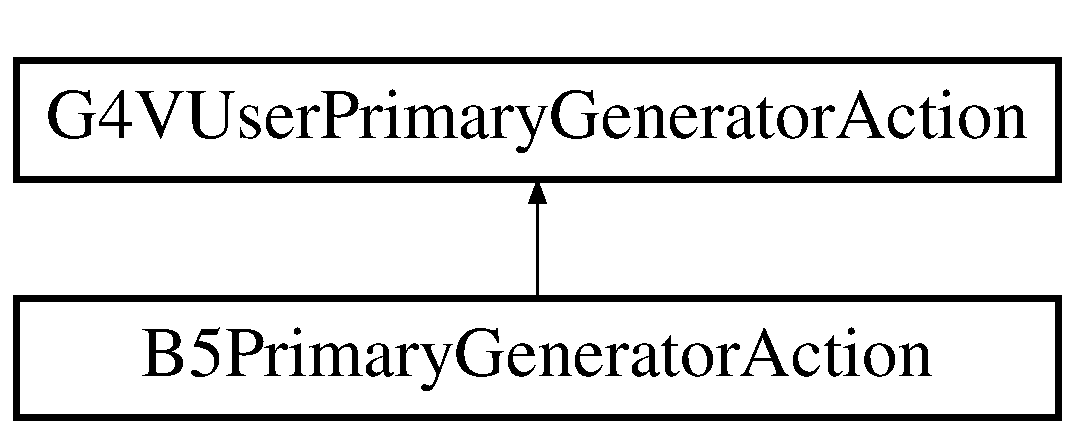
\includegraphics[height=2.000000cm]{class_b5_primary_generator_action}
\end{center}
\end{figure}
\subsection*{Public Member Functions}
\begin{DoxyCompactItemize}
\item 
\hypertarget{class_b5_primary_generator_action_a2a69d1cd59e5f8060a5d830f294d1795}{}virtual void {\bfseries Generate\+Primaries} (G4\+Event $\ast$)\label{class_b5_primary_generator_action_a2a69d1cd59e5f8060a5d830f294d1795}

\item 
\hypertarget{class_b5_primary_generator_action_ad97348ea28b05461d572b853d2dd4d87}{}void {\bfseries Set\+Momentum} (G4double val)\label{class_b5_primary_generator_action_ad97348ea28b05461d572b853d2dd4d87}

\item 
\hypertarget{class_b5_primary_generator_action_abb16b53f40a8ebd6cdbd629ef30a73ba}{}G4double {\bfseries Get\+Momentum} () const \label{class_b5_primary_generator_action_abb16b53f40a8ebd6cdbd629ef30a73ba}

\item 
\hypertarget{class_b5_primary_generator_action_a5fdcff70e700e89b1c27d9532b10a85c}{}void {\bfseries Set\+Sigma\+Momentum} (G4double val)\label{class_b5_primary_generator_action_a5fdcff70e700e89b1c27d9532b10a85c}

\item 
\hypertarget{class_b5_primary_generator_action_ae55153c1ba70382405a8e540f262776c}{}G4double {\bfseries Get\+Sigma\+Momentum} () const \label{class_b5_primary_generator_action_ae55153c1ba70382405a8e540f262776c}

\item 
\hypertarget{class_b5_primary_generator_action_ac5ec2122899938a5322d5797d771d574}{}void {\bfseries Set\+Sigma\+Angle} (G4double val)\label{class_b5_primary_generator_action_ac5ec2122899938a5322d5797d771d574}

\item 
\hypertarget{class_b5_primary_generator_action_a320777d723a43d5868edfe253b438040}{}G4double {\bfseries Get\+Sigma\+Angle} () const \label{class_b5_primary_generator_action_a320777d723a43d5868edfe253b438040}

\item 
\hypertarget{class_b5_primary_generator_action_ab411c002c48e1180008fb00250f22429}{}void {\bfseries Set\+Randomize} (G4bool val)\label{class_b5_primary_generator_action_ab411c002c48e1180008fb00250f22429}

\item 
\hypertarget{class_b5_primary_generator_action_a6d47e2b68f5a0cb43d5a13f15698dda8}{}G4bool {\bfseries Get\+Randomize} () const \label{class_b5_primary_generator_action_a6d47e2b68f5a0cb43d5a13f15698dda8}

\item 
\hypertarget{class_b5_primary_generator_action_a61ea174adaa106e0e5d95b632784b6bb}{}void {\bfseries Set\+Sigma\+Range} (G4double val)\label{class_b5_primary_generator_action_a61ea174adaa106e0e5d95b632784b6bb}

\item 
\hypertarget{class_b5_primary_generator_action_aa48dbf8105aa4b3b67e55a9c51a60d1e}{}G4double {\bfseries Get\+Sigma\+Range} () const \label{class_b5_primary_generator_action_aa48dbf8105aa4b3b67e55a9c51a60d1e}

\item 
\hypertarget{class_b5_primary_generator_action_a0af12d1dd9b918ff127fb964ac2c39d1}{}void {\bfseries Set\+X} (G4double val)\label{class_b5_primary_generator_action_a0af12d1dd9b918ff127fb964ac2c39d1}

\item 
\hypertarget{class_b5_primary_generator_action_a900fe7ff24719adc935860d8d3eb265c}{}G4double {\bfseries Get\+X} () const \label{class_b5_primary_generator_action_a900fe7ff24719adc935860d8d3eb265c}

\item 
\hypertarget{class_b5_primary_generator_action_a8beca0e3506321ceec49776f2d15b201}{}void {\bfseries Set\+Y} (G4double val)\label{class_b5_primary_generator_action_a8beca0e3506321ceec49776f2d15b201}

\item 
\hypertarget{class_b5_primary_generator_action_a4954e13e13ba4da8bef49733795dedd4}{}G4double {\bfseries Get\+Y} () const \label{class_b5_primary_generator_action_a4954e13e13ba4da8bef49733795dedd4}

\item 
\hypertarget{class_b5_primary_generator_action_a7a636bfcd58b5be1f96928769ab1f668}{}void {\bfseries Set\+Z} (G4double val)\label{class_b5_primary_generator_action_a7a636bfcd58b5be1f96928769ab1f668}

\item 
\hypertarget{class_b5_primary_generator_action_a9104fbad5bbdfa9ccaa04850d42540e3}{}G4double {\bfseries Get\+Z} () const \label{class_b5_primary_generator_action_a9104fbad5bbdfa9ccaa04850d42540e3}

\end{DoxyCompactItemize}


\subsection{Detailed Description}
Primary generator

A single particle is generated. User can select
\begin{DoxyItemize}
\item the initial momentum and angle
\item the momentum and angle spreads
\item random selection of a particle type from proton, kaon+, pi+, muon+, e+ 
\end{DoxyItemize}

The documentation for this class was generated from the following files\+:\begin{DoxyCompactItemize}
\item 
\hyperlink{_b5_primary_generator_action_8hh}{B5\+Primary\+Generator\+Action.\+hh}\item 
B5\+Primary\+Generator\+Action.\+cc\end{DoxyCompactItemize}

\hypertarget{class_ex_n04_primary_generator_action}{}\section{Ex\+N04\+Primary\+Generator\+Action Class Reference}
\label{class_ex_n04_primary_generator_action}\index{Ex\+N04\+Primary\+Generator\+Action@{Ex\+N04\+Primary\+Generator\+Action}}
Inheritance diagram for Ex\+N04\+Primary\+Generator\+Action\+:\begin{figure}[H]
\begin{center}
\leavevmode
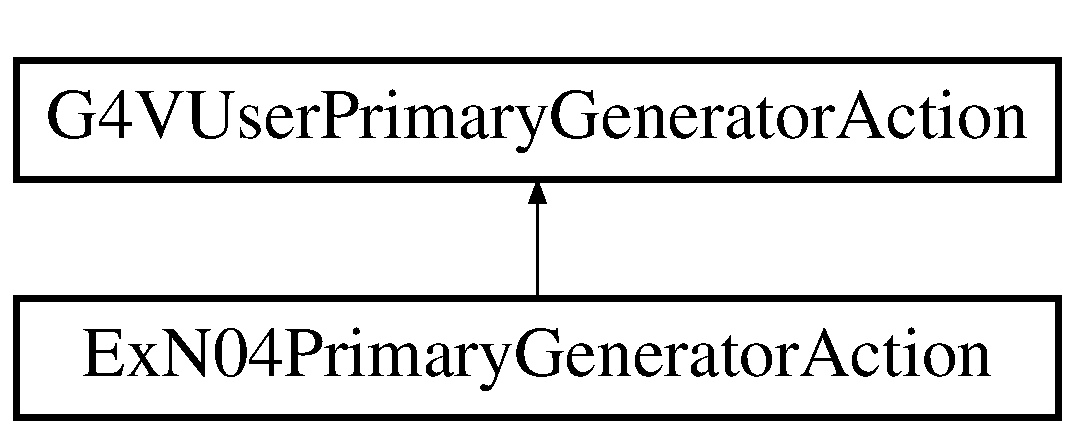
\includegraphics[height=2.000000cm]{class_ex_n04_primary_generator_action}
\end{center}
\end{figure}
\subsection*{Public Member Functions}
\begin{DoxyCompactItemize}
\item 
\hypertarget{class_ex_n04_primary_generator_action_a9aad116df9cd1f2fa5ec26b7faba7eb0}{}virtual void {\bfseries Generate\+Primaries} (G4\+Event $\ast$an\+Event)\label{class_ex_n04_primary_generator_action_a9aad116df9cd1f2fa5ec26b7faba7eb0}

\item 
\hypertarget{class_ex_n04_primary_generator_action_aff8fb2ce7b737b6e9242f6fcb506e82d}{}void {\bfseries Set\+Generator} (G4\+V\+Primary\+Generator $\ast$gen)\label{class_ex_n04_primary_generator_action_aff8fb2ce7b737b6e9242f6fcb506e82d}

\item 
\hypertarget{class_ex_n04_primary_generator_action_a0f9df527485e34679aad0708212f6d42}{}void {\bfseries Set\+Generator} (G4\+String genname)\label{class_ex_n04_primary_generator_action_a0f9df527485e34679aad0708212f6d42}

\item 
\hypertarget{class_ex_n04_primary_generator_action_ac055f78ed9d64550d728ec91d589e2b3}{}G4\+V\+Primary\+Generator $\ast$ {\bfseries Get\+Generator} () const \label{class_ex_n04_primary_generator_action_ac055f78ed9d64550d728ec91d589e2b3}

\item 
\hypertarget{class_ex_n04_primary_generator_action_a3f46e479a8104e6cd1f5b701345fb3eb}{}G4\+String {\bfseries Get\+Generator\+Name} () const \label{class_ex_n04_primary_generator_action_a3f46e479a8104e6cd1f5b701345fb3eb}

\end{DoxyCompactItemize}


The documentation for this class was generated from the following files\+:\begin{DoxyCompactItemize}
\item 
Ex\+N04\+Primary\+Generator\+Action.\+hh\item 
Ex\+N04\+Primary\+Generator\+Action.\+cc\end{DoxyCompactItemize}

\hypertarget{class_ex_n04_primary_generator_messenger}{}\section{Ex\+N04\+Primary\+Generator\+Messenger Class Reference}
\label{class_ex_n04_primary_generator_messenger}\index{Ex\+N04\+Primary\+Generator\+Messenger@{Ex\+N04\+Primary\+Generator\+Messenger}}
Inheritance diagram for Ex\+N04\+Primary\+Generator\+Messenger\+:\begin{figure}[H]
\begin{center}
\leavevmode
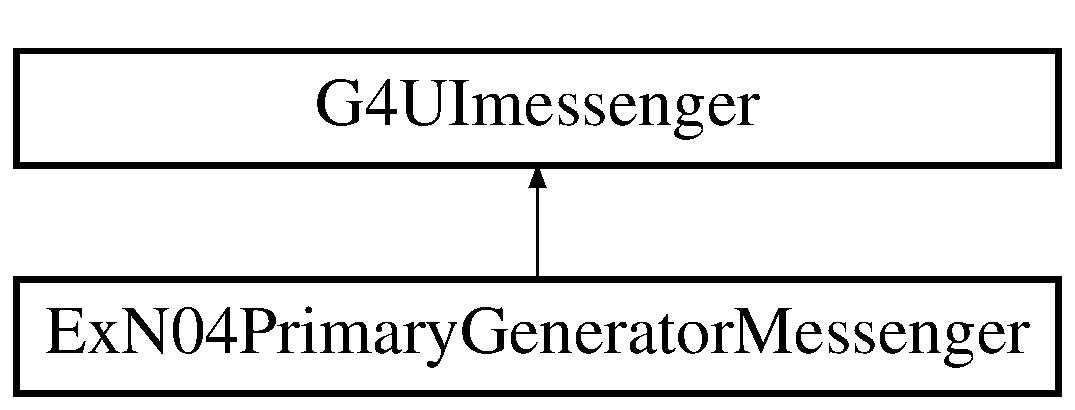
\includegraphics[height=2.000000cm]{class_ex_n04_primary_generator_messenger}
\end{center}
\end{figure}
\subsection*{Public Member Functions}
\begin{DoxyCompactItemize}
\item 
\hypertarget{class_ex_n04_primary_generator_messenger_aaf4263c261782080d07ca993ba7ee6e2}{}{\bfseries Ex\+N04\+Primary\+Generator\+Messenger} (\hyperlink{class_ex_n04_primary_generator_action}{Ex\+N04\+Primary\+Generator\+Action} $\ast$genaction)\label{class_ex_n04_primary_generator_messenger_aaf4263c261782080d07ca993ba7ee6e2}

\item 
\hypertarget{class_ex_n04_primary_generator_messenger_a4419691c4e4267b5075965ca19b5443e}{}void {\bfseries Set\+New\+Value} (G4\+U\+Icommand $\ast$command, G4\+String new\+Values)\label{class_ex_n04_primary_generator_messenger_a4419691c4e4267b5075965ca19b5443e}

\item 
\hypertarget{class_ex_n04_primary_generator_messenger_a3fe369aa5dc19e59bc8bbfb8db33c34f}{}G4\+String {\bfseries Get\+Current\+Value} (G4\+U\+Icommand $\ast$command)\label{class_ex_n04_primary_generator_messenger_a3fe369aa5dc19e59bc8bbfb8db33c34f}

\end{DoxyCompactItemize}


The documentation for this class was generated from the following files\+:\begin{DoxyCompactItemize}
\item 
Ex\+N04\+Primary\+Generator\+Messenger.\+hh\item 
Ex\+N04\+Primary\+Generator\+Messenger.\+cc\end{DoxyCompactItemize}

\hypertarget{structhepevt}{}\section{hepevt Struct Reference}
\label{structhepevt}\index{hepevt@{hepevt}}
\subsection*{Public Attributes}
\begin{DoxyCompactItemize}
\item 
\hypertarget{structhepevt_aa52f667afe96b88afb75e90bba01c6dd}{}char {\bfseries data} \mbox{[}hepevt\+\_\+bytes\+\_\+allocation\mbox{]}\label{structhepevt_aa52f667afe96b88afb75e90bba01c6dd}

\end{DoxyCompactItemize}


The documentation for this struct was generated from the following file\+:\begin{DoxyCompactItemize}
\item 
H\+E\+P\+Evtcom.\+cc\end{DoxyCompactItemize}

\hypertarget{class_hep_m_c_g4_ascii_reader}{}\section{Hep\+M\+C\+G4\+Ascii\+Reader Class Reference}
\label{class_hep_m_c_g4_ascii_reader}\index{Hep\+M\+C\+G4\+Ascii\+Reader@{Hep\+M\+C\+G4\+Ascii\+Reader}}
Inheritance diagram for Hep\+M\+C\+G4\+Ascii\+Reader\+:\begin{figure}[H]
\begin{center}
\leavevmode
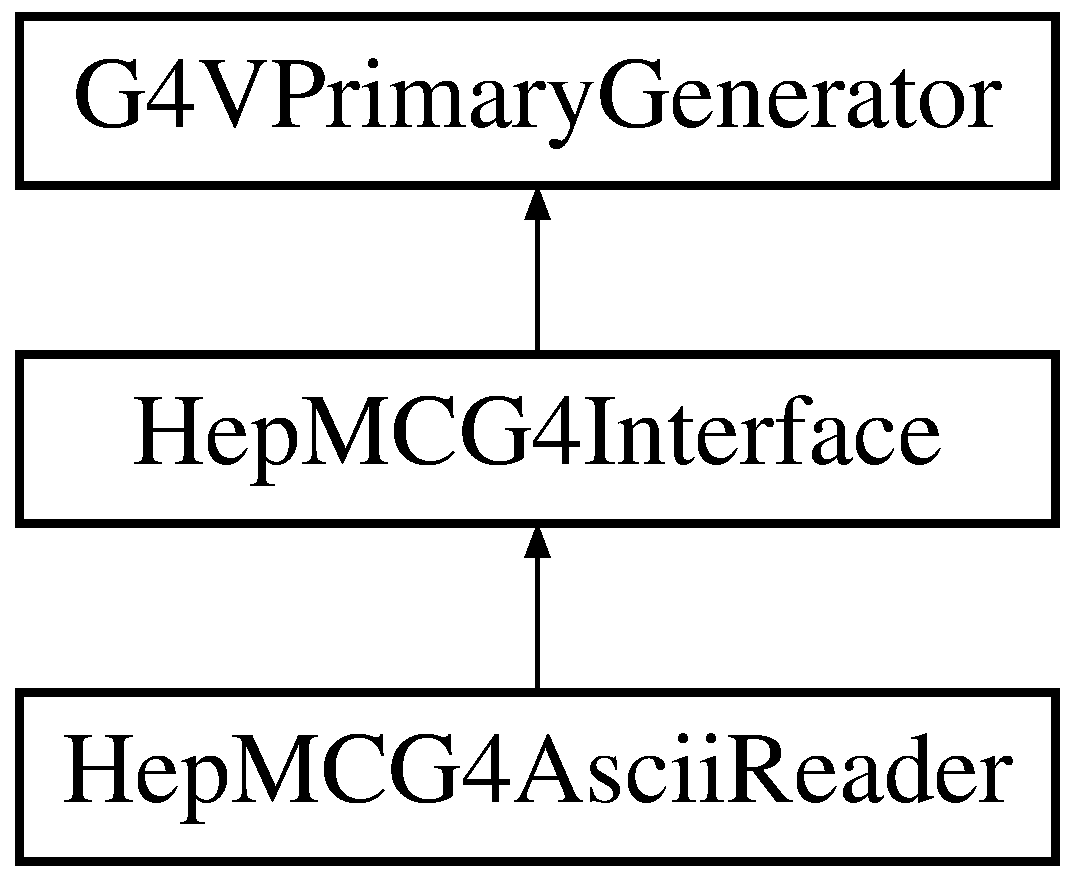
\includegraphics[height=3.000000cm]{class_hep_m_c_g4_ascii_reader}
\end{center}
\end{figure}
\subsection*{Public Member Functions}
\begin{DoxyCompactItemize}
\item 
\hypertarget{class_hep_m_c_g4_ascii_reader_a5063529b9bb4b313ee06e22586a65307}{}void {\bfseries Set\+File\+Name} (G4\+String name)\label{class_hep_m_c_g4_ascii_reader_a5063529b9bb4b313ee06e22586a65307}

\item 
\hypertarget{class_hep_m_c_g4_ascii_reader_a5a9220dfa44114171c1ed8f73e8877fc}{}G4\+String {\bfseries Get\+File\+Name} () const \label{class_hep_m_c_g4_ascii_reader_a5a9220dfa44114171c1ed8f73e8877fc}

\item 
\hypertarget{class_hep_m_c_g4_ascii_reader_a900843ac4f5da113a1ad788656747478}{}void {\bfseries Set\+Verbose\+Level} (G4int i)\label{class_hep_m_c_g4_ascii_reader_a900843ac4f5da113a1ad788656747478}

\item 
\hypertarget{class_hep_m_c_g4_ascii_reader_a71f59f07680ca33a5d532d47147a036a}{}G4int {\bfseries Get\+Verbose\+Level} () const \label{class_hep_m_c_g4_ascii_reader_a71f59f07680ca33a5d532d47147a036a}

\item 
\hypertarget{class_hep_m_c_g4_ascii_reader_adff7c9489d2d6958cdca4ed49fdaac68}{}void {\bfseries Initialize} ()\label{class_hep_m_c_g4_ascii_reader_adff7c9489d2d6958cdca4ed49fdaac68}

\end{DoxyCompactItemize}
\subsection*{Protected Member Functions}
\begin{DoxyCompactItemize}
\item 
\hypertarget{class_hep_m_c_g4_ascii_reader_a77b49168d34bbd03923be535c3e695e4}{}virtual Hep\+M\+C\+::\+Gen\+Event $\ast$ {\bfseries Generate\+Hep\+M\+C\+Event} ()\label{class_hep_m_c_g4_ascii_reader_a77b49168d34bbd03923be535c3e695e4}

\end{DoxyCompactItemize}
\subsection*{Protected Attributes}
\begin{DoxyCompactItemize}
\item 
\hypertarget{class_hep_m_c_g4_ascii_reader_aefd38d468f9894b503385d2d9b7be11d}{}G4\+String {\bfseries filename}\label{class_hep_m_c_g4_ascii_reader_aefd38d468f9894b503385d2d9b7be11d}

\item 
\hypertarget{class_hep_m_c_g4_ascii_reader_a4ea809bbcdcb48fddfdc508696a932a6}{}Hep\+M\+C\+::\+I\+O\+\_\+\+Gen\+Event $\ast$ {\bfseries ascii\+Input}\label{class_hep_m_c_g4_ascii_reader_a4ea809bbcdcb48fddfdc508696a932a6}

\item 
\hypertarget{class_hep_m_c_g4_ascii_reader_a13c4641c3d9c5d24ba8c028e79abb0ed}{}G4int {\bfseries verbose}\label{class_hep_m_c_g4_ascii_reader_a13c4641c3d9c5d24ba8c028e79abb0ed}

\item 
\hypertarget{class_hep_m_c_g4_ascii_reader_a5b6338d96b9c64492bdc1c87d7070cb8}{}\hyperlink{class_hep_m_c_g4_ascii_reader_messenger}{Hep\+M\+C\+G4\+Ascii\+Reader\+Messenger} $\ast$ {\bfseries messenger}\label{class_hep_m_c_g4_ascii_reader_a5b6338d96b9c64492bdc1c87d7070cb8}

\end{DoxyCompactItemize}


The documentation for this class was generated from the following files\+:\begin{DoxyCompactItemize}
\item 
Hep\+M\+C\+G4\+Ascii\+Reader.\+hh\item 
Hep\+M\+C\+G4\+Ascii\+Reader.\+cc\end{DoxyCompactItemize}

\hypertarget{class_hep_m_c_g4_ascii_reader_messenger}{}\section{Hep\+M\+C\+G4\+Ascii\+Reader\+Messenger Class Reference}
\label{class_hep_m_c_g4_ascii_reader_messenger}\index{Hep\+M\+C\+G4\+Ascii\+Reader\+Messenger@{Hep\+M\+C\+G4\+Ascii\+Reader\+Messenger}}
Inheritance diagram for Hep\+M\+C\+G4\+Ascii\+Reader\+Messenger\+:\begin{figure}[H]
\begin{center}
\leavevmode
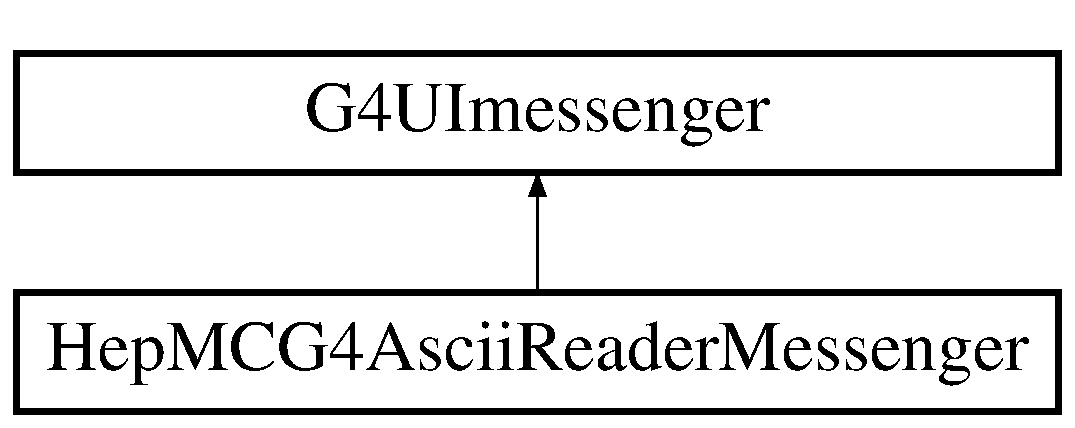
\includegraphics[height=2.000000cm]{class_hep_m_c_g4_ascii_reader_messenger}
\end{center}
\end{figure}
\subsection*{Public Member Functions}
\begin{DoxyCompactItemize}
\item 
\hypertarget{class_hep_m_c_g4_ascii_reader_messenger_ad5d0392af95284f57b95244390c17f35}{}{\bfseries Hep\+M\+C\+G4\+Ascii\+Reader\+Messenger} (\hyperlink{class_hep_m_c_g4_ascii_reader}{Hep\+M\+C\+G4\+Ascii\+Reader} $\ast$agen)\label{class_hep_m_c_g4_ascii_reader_messenger_ad5d0392af95284f57b95244390c17f35}

\item 
\hypertarget{class_hep_m_c_g4_ascii_reader_messenger_ab7cbaf09ff5ed12bb49d8be46467b37c}{}void {\bfseries Set\+New\+Value} (G4\+U\+Icommand $\ast$command, G4\+String new\+Values)\label{class_hep_m_c_g4_ascii_reader_messenger_ab7cbaf09ff5ed12bb49d8be46467b37c}

\item 
\hypertarget{class_hep_m_c_g4_ascii_reader_messenger_ad60e3f13f83fb90656676d3087d30ffd}{}G4\+String {\bfseries Get\+Current\+Value} (G4\+U\+Icommand $\ast$command)\label{class_hep_m_c_g4_ascii_reader_messenger_ad60e3f13f83fb90656676d3087d30ffd}

\end{DoxyCompactItemize}


The documentation for this class was generated from the following files\+:\begin{DoxyCompactItemize}
\item 
Hep\+M\+C\+G4\+Ascii\+Reader\+Messenger.\+hh\item 
Hep\+M\+C\+G4\+Ascii\+Reader\+Messenger.\+cc\end{DoxyCompactItemize}

\hypertarget{class_hep_m_c_g4_interface}{}\section{Hep\+M\+C\+G4\+Interface Class Reference}
\label{class_hep_m_c_g4_interface}\index{Hep\+M\+C\+G4\+Interface@{Hep\+M\+C\+G4\+Interface}}


{\ttfamily \#include $<$Hep\+M\+C\+G4\+Interface.\+hh$>$}

Inheritance diagram for Hep\+M\+C\+G4\+Interface\+:\begin{figure}[H]
\begin{center}
\leavevmode
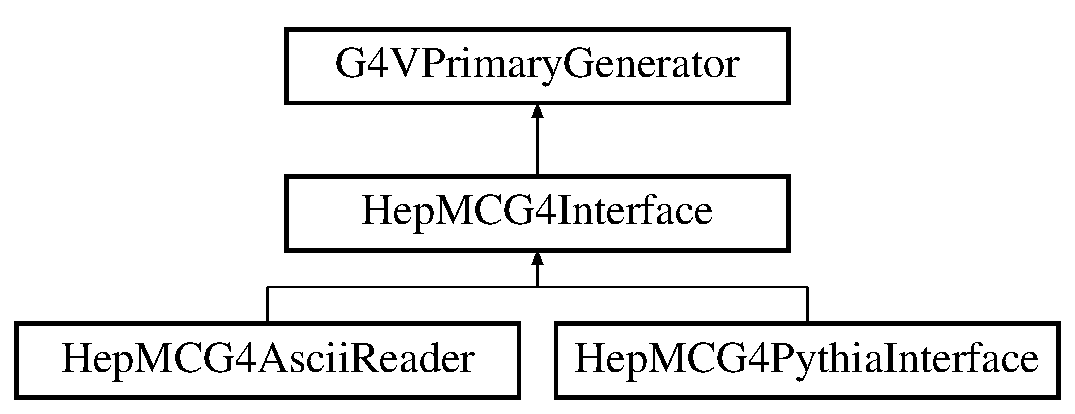
\includegraphics[height=3.000000cm]{class_hep_m_c_g4_interface}
\end{center}
\end{figure}
\subsection*{Public Member Functions}
\begin{DoxyCompactItemize}
\item 
\hypertarget{class_hep_m_c_g4_interface_a0e9f3cae6c2d9ef27619a6db8af39c58}{}Hep\+M\+C\+::\+Gen\+Event $\ast$ {\bfseries Get\+Hep\+M\+C\+Gen\+Event} () const \label{class_hep_m_c_g4_interface_a0e9f3cae6c2d9ef27619a6db8af39c58}

\item 
\hypertarget{class_hep_m_c_g4_interface_a2947defb50b862d5fe962ebd35b35b3b}{}virtual void {\bfseries Generate\+Primary\+Vertex} (G4\+Event $\ast$an\+Event)\label{class_hep_m_c_g4_interface_a2947defb50b862d5fe962ebd35b35b3b}

\end{DoxyCompactItemize}
\subsection*{Protected Member Functions}
\begin{DoxyCompactItemize}
\item 
\hypertarget{class_hep_m_c_g4_interface_aa6506443875a8f04967dc28f0941bedf}{}virtual G4bool {\bfseries Check\+Vertex\+Inside\+World} (const G4\+Three\+Vector \&pos) const \label{class_hep_m_c_g4_interface_aa6506443875a8f04967dc28f0941bedf}

\item 
\hypertarget{class_hep_m_c_g4_interface_a40b29a7630cc2aa89f16a6ef104a03b6}{}void {\bfseries Hep\+M\+C2\+G4} (const Hep\+M\+C\+::\+Gen\+Event $\ast$hepmcevt, G4\+Event $\ast$g4event)\label{class_hep_m_c_g4_interface_a40b29a7630cc2aa89f16a6ef104a03b6}

\item 
\hypertarget{class_hep_m_c_g4_interface_a5f04579412ea7f076b319e209d048c07}{}virtual Hep\+M\+C\+::\+Gen\+Event $\ast$ {\bfseries Generate\+Hep\+M\+C\+Event} ()\label{class_hep_m_c_g4_interface_a5f04579412ea7f076b319e209d048c07}

\end{DoxyCompactItemize}
\subsection*{Protected Attributes}
\begin{DoxyCompactItemize}
\item 
\hypertarget{class_hep_m_c_g4_interface_af25ddb31c0fd20eaa528c42c74a57361}{}Hep\+M\+C\+::\+Gen\+Event $\ast$ {\bfseries hepmc\+Event}\label{class_hep_m_c_g4_interface_af25ddb31c0fd20eaa528c42c74a57361}

\end{DoxyCompactItemize}


\subsection{Detailed Description}
A base class for primary generation via Hep\+M\+C object. This class is derived from G4\+V\+Primary\+Generator. 

The documentation for this class was generated from the following files\+:\begin{DoxyCompactItemize}
\item 
Hep\+M\+C\+G4\+Interface.\+hh\item 
Hep\+M\+C\+G4\+Interface.\+cc\end{DoxyCompactItemize}

\hypertarget{class_hep_m_c_g4_pythia_interface}{}\section{Hep\+M\+C\+G4\+Pythia\+Interface Class Reference}
\label{class_hep_m_c_g4_pythia_interface}\index{Hep\+M\+C\+G4\+Pythia\+Interface@{Hep\+M\+C\+G4\+Pythia\+Interface}}


A generic interface class with Pythia event generator via Hep\+M\+C.  




{\ttfamily \#include $<$Hep\+M\+C\+G4\+Pythia\+Interface.\+hh$>$}

Inheritance diagram for Hep\+M\+C\+G4\+Pythia\+Interface\+:\begin{figure}[H]
\begin{center}
\leavevmode
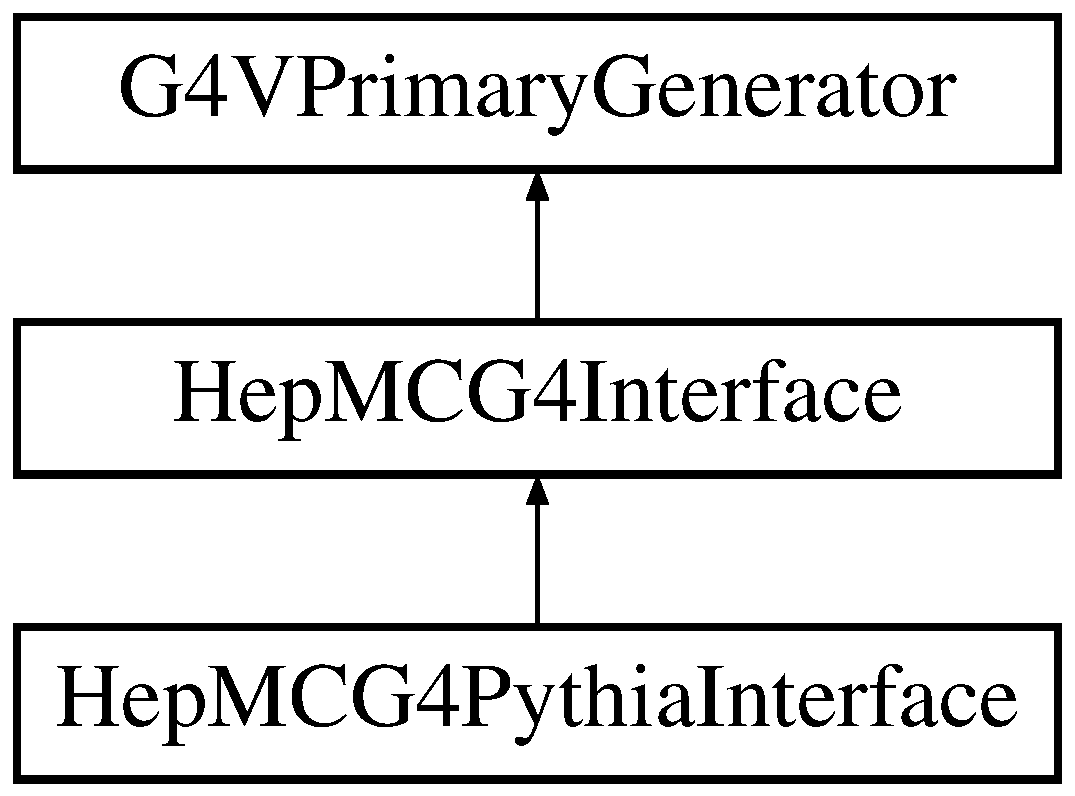
\includegraphics[height=3.000000cm]{class_hep_m_c_g4_pythia_interface}
\end{center}
\end{figure}
\subsection*{Public Member Functions}
\begin{DoxyCompactItemize}
\item 
\hypertarget{class_hep_m_c_g4_pythia_interface_a6bebc88001f05ded58041b4f0426926f}{}void {\bfseries Set\+Verbose\+Level} (G4int i)\label{class_hep_m_c_g4_pythia_interface_a6bebc88001f05ded58041b4f0426926f}

\item 
\hypertarget{class_hep_m_c_g4_pythia_interface_abf6c19f7c69d397cef873502ae387531}{}G4int {\bfseries Get\+Verbose\+Level} () const \label{class_hep_m_c_g4_pythia_interface_abf6c19f7c69d397cef873502ae387531}

\item 
\hypertarget{class_hep_m_c_g4_pythia_interface_a5cf44f1b169369fed4a0456901867c2d}{}void {\bfseries Set\+Pylist} (G4int i)\label{class_hep_m_c_g4_pythia_interface_a5cf44f1b169369fed4a0456901867c2d}

\item 
\hypertarget{class_hep_m_c_g4_pythia_interface_a41f2d519af2273d7b99b5eb62e67894d}{}G4int {\bfseries Get\+Pylist} () const \label{class_hep_m_c_g4_pythia_interface_a41f2d519af2273d7b99b5eb62e67894d}

\item 
\hypertarget{class_hep_m_c_g4_pythia_interface_a5b8d73fc3d65b4539cfca4168101ce14}{}void {\bfseries Call\+Pyinit} (G4\+String frame, G4\+String beam, G4\+String target, G4double win)\label{class_hep_m_c_g4_pythia_interface_a5b8d73fc3d65b4539cfca4168101ce14}

\item 
\hypertarget{class_hep_m_c_g4_pythia_interface_a7f853e52f16a3fba0265380932c9cf43}{}void {\bfseries Call\+Pystat} (G4int istat)\label{class_hep_m_c_g4_pythia_interface_a7f853e52f16a3fba0265380932c9cf43}

\item 
\hypertarget{class_hep_m_c_g4_pythia_interface_a609e892870a9592cdea8be836c21573c}{}void {\bfseries Set\+Random\+Seed} (G4int iseed)\label{class_hep_m_c_g4_pythia_interface_a609e892870a9592cdea8be836c21573c}

\item 
\hypertarget{class_hep_m_c_g4_pythia_interface_ae8163e7f051487ed2284dd89d0c6890d}{}void {\bfseries Call\+Pygive} (G4\+String par)\label{class_hep_m_c_g4_pythia_interface_ae8163e7f051487ed2284dd89d0c6890d}

\item 
\hypertarget{class_hep_m_c_g4_pythia_interface_ae61079ec925b5d7ba40bae6e8dda09ea}{}void {\bfseries Call\+Pyrget} (G4int lun, G4int move)\label{class_hep_m_c_g4_pythia_interface_ae61079ec925b5d7ba40bae6e8dda09ea}

\item 
\hypertarget{class_hep_m_c_g4_pythia_interface_a250ad0eb10834f554314fae10b454710}{}void {\bfseries Call\+Pyrset} (G4int lun, G4int move)\label{class_hep_m_c_g4_pythia_interface_a250ad0eb10834f554314fae10b454710}

\item 
\hypertarget{class_hep_m_c_g4_pythia_interface_abdb8a01a6157c91de6bff2177a4cf3fd}{}void {\bfseries Print\+Random\+Status} (std\+::ostream \&ostr=G4cout) const \label{class_hep_m_c_g4_pythia_interface_abdb8a01a6157c91de6bff2177a4cf3fd}

\item 
\hypertarget{class_hep_m_c_g4_pythia_interface_aa17ddba03c246a9f0011c31a3a601b24}{}virtual void {\bfseries Set\+User\+Parameters} ()\label{class_hep_m_c_g4_pythia_interface_aa17ddba03c246a9f0011c31a3a601b24}

\item 
\hypertarget{class_hep_m_c_g4_pythia_interface_a01e0ffc1f48ee73cde6f1a7af383db17}{}virtual void {\bfseries Print} () const \label{class_hep_m_c_g4_pythia_interface_a01e0ffc1f48ee73cde6f1a7af383db17}

\end{DoxyCompactItemize}
\subsection*{Protected Member Functions}
\begin{DoxyCompactItemize}
\item 
\hypertarget{class_hep_m_c_g4_pythia_interface_a35f96ffb6e7e846e1784321a87aa4859}{}virtual Hep\+M\+C\+::\+Gen\+Event $\ast$ {\bfseries Generate\+Hep\+M\+C\+Event} ()\label{class_hep_m_c_g4_pythia_interface_a35f96ffb6e7e846e1784321a87aa4859}

\end{DoxyCompactItemize}
\subsection*{Protected Attributes}
\begin{DoxyCompactItemize}
\item 
\hypertarget{class_hep_m_c_g4_pythia_interface_a53097ae82a7f0288e75c063679579d64}{}G4int {\bfseries verbose}\label{class_hep_m_c_g4_pythia_interface_a53097ae82a7f0288e75c063679579d64}

\item 
\hypertarget{class_hep_m_c_g4_pythia_interface_a327b9fdcde2ff2601ceccf1650a4fb48}{}G4int {\bfseries mpylist}\label{class_hep_m_c_g4_pythia_interface_a327b9fdcde2ff2601ceccf1650a4fb48}

\item 
\hypertarget{class_hep_m_c_g4_pythia_interface_a5aa2077f91e9bd75e551bca38742046e}{}Hep\+M\+C\+::\+I\+O\+\_\+\+H\+E\+P\+E\+V\+T {\bfseries hepevtio}\label{class_hep_m_c_g4_pythia_interface_a5aa2077f91e9bd75e551bca38742046e}

\item 
\hypertarget{class_hep_m_c_g4_pythia_interface_ac0541688df49e9ba60bd7771000eb483}{}\hyperlink{class_hep_m_c_g4_pythia_messenger}{Hep\+M\+C\+G4\+Pythia\+Messenger} $\ast$ {\bfseries messenger}\label{class_hep_m_c_g4_pythia_interface_ac0541688df49e9ba60bd7771000eb483}

\end{DoxyCompactItemize}


\subsection{Detailed Description}
A generic interface class with Pythia event generator via Hep\+M\+C. 

The documentation for this class was generated from the following file\+:\begin{DoxyCompactItemize}
\item 
Hep\+M\+C\+G4\+Pythia\+Interface.\+hh\end{DoxyCompactItemize}

\hypertarget{class_hep_m_c_g4_pythia_messenger}{}\section{Hep\+M\+C\+G4\+Pythia\+Messenger Class Reference}
\label{class_hep_m_c_g4_pythia_messenger}\index{Hep\+M\+C\+G4\+Pythia\+Messenger@{Hep\+M\+C\+G4\+Pythia\+Messenger}}
Inheritance diagram for Hep\+M\+C\+G4\+Pythia\+Messenger\+:\begin{figure}[H]
\begin{center}
\leavevmode
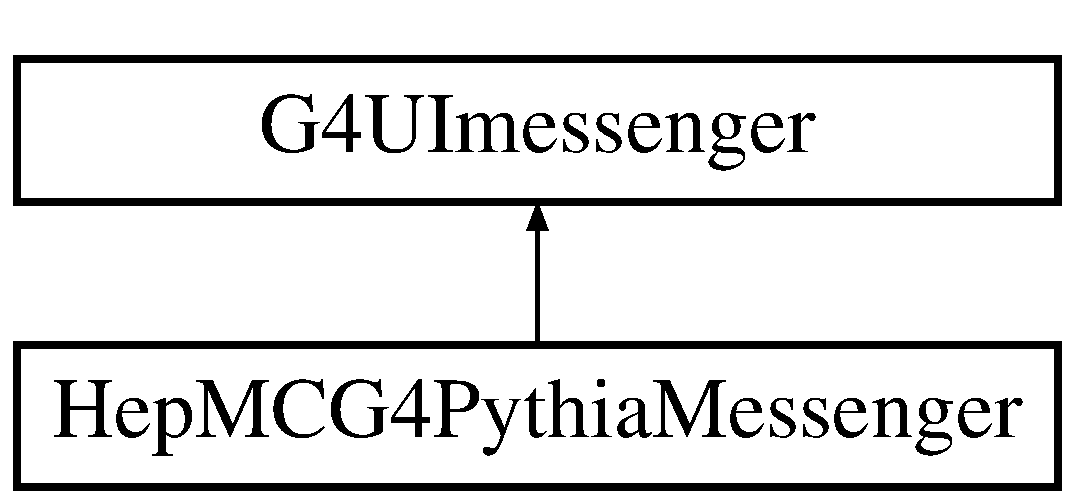
\includegraphics[height=2.000000cm]{class_hep_m_c_g4_pythia_messenger}
\end{center}
\end{figure}
\subsection*{Public Member Functions}
\begin{DoxyCompactItemize}
\item 
\hypertarget{class_hep_m_c_g4_pythia_messenger_a58ebd7ec73e23a7a7e1001e64a5f6720}{}{\bfseries Hep\+M\+C\+G4\+Pythia\+Messenger} (\hyperlink{class_hep_m_c_g4_pythia_interface}{Hep\+M\+C\+G4\+Pythia\+Interface} $\ast$agen)\label{class_hep_m_c_g4_pythia_messenger_a58ebd7ec73e23a7a7e1001e64a5f6720}

\item 
\hypertarget{class_hep_m_c_g4_pythia_messenger_a5956a14ab047c10b65de9317389f8b57}{}void {\bfseries Set\+New\+Value} (G4\+U\+Icommand $\ast$command, G4\+String new\+Values)\label{class_hep_m_c_g4_pythia_messenger_a5956a14ab047c10b65de9317389f8b57}

\item 
\hypertarget{class_hep_m_c_g4_pythia_messenger_aa38cadfb3089bcaf970a515546daeff6}{}G4\+String {\bfseries Get\+Current\+Value} (G4\+U\+Icommand $\ast$command)\label{class_hep_m_c_g4_pythia_messenger_aa38cadfb3089bcaf970a515546daeff6}

\end{DoxyCompactItemize}


The documentation for this class was generated from the following file\+:\begin{DoxyCompactItemize}
\item 
Hep\+M\+C\+G4\+Pythia\+Messenger.\+hh\end{DoxyCompactItemize}

\hypertarget{class_magnetic_field}{}\section{Magnetic\+Field Class Reference}
\label{class_magnetic_field}\index{Magnetic\+Field@{Magnetic\+Field}}


Magnetic field.  




{\ttfamily \#include $<$Magnetic\+Field.\+hh$>$}

Inheritance diagram for Magnetic\+Field\+:\begin{figure}[H]
\begin{center}
\leavevmode
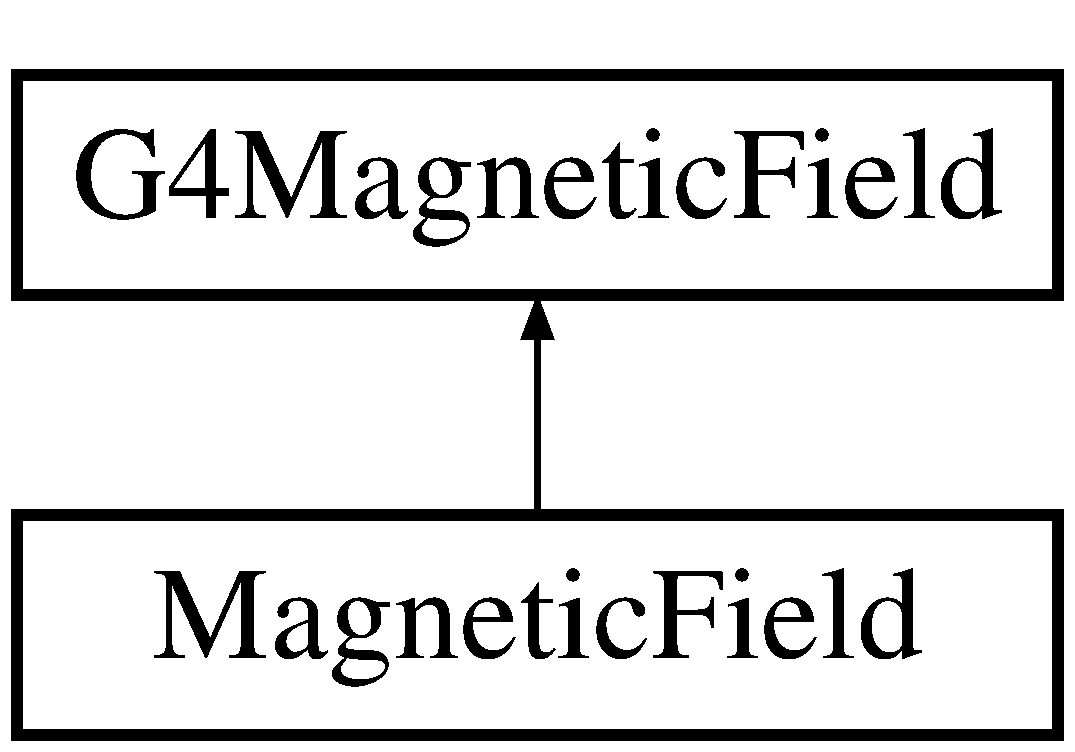
\includegraphics[height=2.000000cm]{class_magnetic_field}
\end{center}
\end{figure}
\subsection*{Public Member Functions}
\begin{DoxyCompactItemize}
\item 
\hypertarget{class_magnetic_field_abe1e09a803c7a4dd4ba309b2a812b18c}{}virtual void {\bfseries Get\+Field\+Value} (const G4double point\mbox{[}4\mbox{]}, double $\ast$b\+Field) const \label{class_magnetic_field_abe1e09a803c7a4dd4ba309b2a812b18c}

\item 
\hypertarget{class_magnetic_field_a252b22b09dff47a404b209568716288b}{}void {\bfseries Set\+Field} (G4double val)\label{class_magnetic_field_a252b22b09dff47a404b209568716288b}

\item 
\hypertarget{class_magnetic_field_a6254a001c9505fbdcc7c3270e9e58e78}{}G4double {\bfseries Get\+Field} () const \label{class_magnetic_field_a6254a001c9505fbdcc7c3270e9e58e78}

\end{DoxyCompactItemize}


\subsection{Detailed Description}
Magnetic field. 

The documentation for this class was generated from the following files\+:\begin{DoxyCompactItemize}
\item 
Magnetic\+Field.\+hh\item 
Magnetic\+Field.\+cc\end{DoxyCompactItemize}

\hypertarget{class_r_h_i_c_f_action_initialization}{}\section{R\+H\+I\+C\+F\+Action\+Initialization Class Reference}
\label{class_r_h_i_c_f_action_initialization}\index{R\+H\+I\+C\+F\+Action\+Initialization@{R\+H\+I\+C\+F\+Action\+Initialization}}


Action initialization class.  




{\ttfamily \#include $<$R\+H\+I\+C\+F\+Action\+Initialization.\+hh$>$}

Inheritance diagram for R\+H\+I\+C\+F\+Action\+Initialization\+:\begin{figure}[H]
\begin{center}
\leavevmode
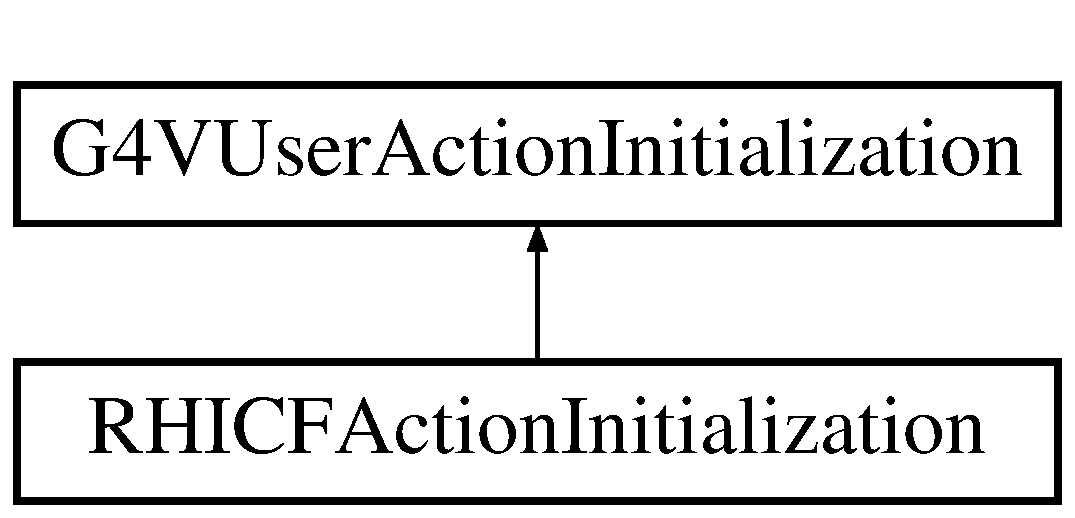
\includegraphics[height=2.000000cm]{class_r_h_i_c_f_action_initialization}
\end{center}
\end{figure}
\subsection*{Public Member Functions}
\begin{DoxyCompactItemize}
\item 
\hypertarget{class_r_h_i_c_f_action_initialization_a924cf44864114ca218a5901b153fde12}{}virtual void {\bfseries Build\+For\+Master} () const \label{class_r_h_i_c_f_action_initialization_a924cf44864114ca218a5901b153fde12}

\item 
\hypertarget{class_r_h_i_c_f_action_initialization_aca5ab38c02f02f18eddf39fe05936719}{}virtual void {\bfseries Build} () const \label{class_r_h_i_c_f_action_initialization_aca5ab38c02f02f18eddf39fe05936719}

\end{DoxyCompactItemize}


\subsection{Detailed Description}
Action initialization class. 

The documentation for this class was generated from the following files\+:\begin{DoxyCompactItemize}
\item 
R\+H\+I\+C\+F\+Action\+Initialization.\+hh\item 
R\+H\+I\+C\+F\+Action\+Initialization.\+cc\end{DoxyCompactItemize}

\hypertarget{class_r_h_i_c_f_detector_construction}{}\section{R\+H\+I\+C\+F\+Detector\+Construction Class Reference}
\label{class_r_h_i_c_f_detector_construction}\index{R\+H\+I\+C\+F\+Detector\+Construction@{R\+H\+I\+C\+F\+Detector\+Construction}}
Inheritance diagram for R\+H\+I\+C\+F\+Detector\+Construction\+:\begin{figure}[H]
\begin{center}
\leavevmode
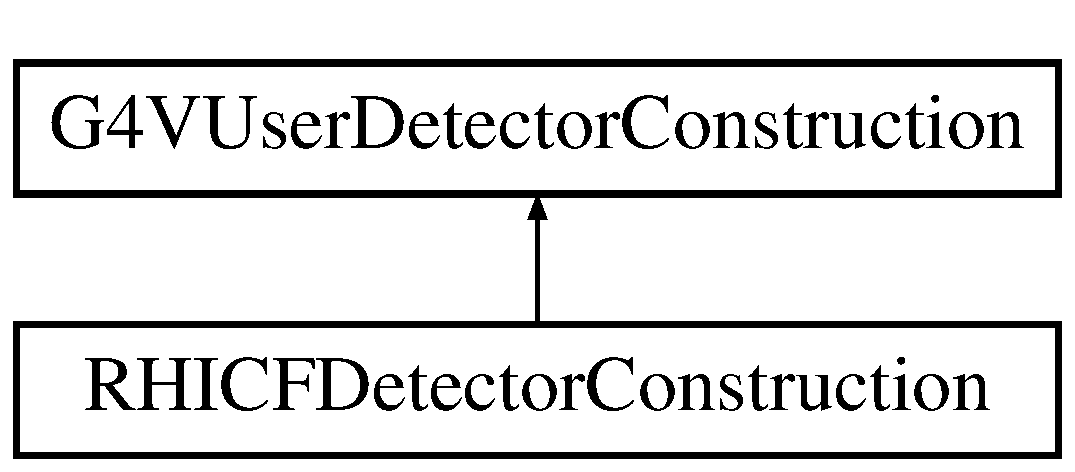
\includegraphics[height=2.000000cm]{class_r_h_i_c_f_detector_construction}
\end{center}
\end{figure}
\subsection*{Public Member Functions}
\begin{DoxyCompactItemize}
\item 
\hypertarget{class_r_h_i_c_f_detector_construction_ac57e59ee13d87e7a6c6d46566139f431}{}virtual G4\+V\+Physical\+Volume $\ast$ {\bfseries Construct} ()\label{class_r_h_i_c_f_detector_construction_ac57e59ee13d87e7a6c6d46566139f431}

\item 
\hypertarget{class_r_h_i_c_f_detector_construction_a7a867fd39f284639fcca381f5d4e50b9}{}virtual void {\bfseries Construct\+S\+Dand\+Field} ()\label{class_r_h_i_c_f_detector_construction_a7a867fd39f284639fcca381f5d4e50b9}

\item 
\hypertarget{class_r_h_i_c_f_detector_construction_a9caa382d52787d0e95743197103061db}{}G4\+Material $\ast$ {\bfseries Find\+Material} (G4\+String)\label{class_r_h_i_c_f_detector_construction_a9caa382d52787d0e95743197103061db}

\end{DoxyCompactItemize}


The documentation for this class was generated from the following files\+:\begin{DoxyCompactItemize}
\item 
R\+H\+I\+C\+F\+Detector\+Construction.\+hh\item 
R\+H\+I\+C\+F\+Detector\+Construction.\+cc\end{DoxyCompactItemize}

\hypertarget{class_r_h_i_c_f_event_action}{}\section{R\+H\+I\+C\+F\+Event\+Action Class Reference}
\label{class_r_h_i_c_f_event_action}\index{R\+H\+I\+C\+F\+Event\+Action@{R\+H\+I\+C\+F\+Event\+Action}}
Inheritance diagram for R\+H\+I\+C\+F\+Event\+Action\+:\begin{figure}[H]
\begin{center}
\leavevmode
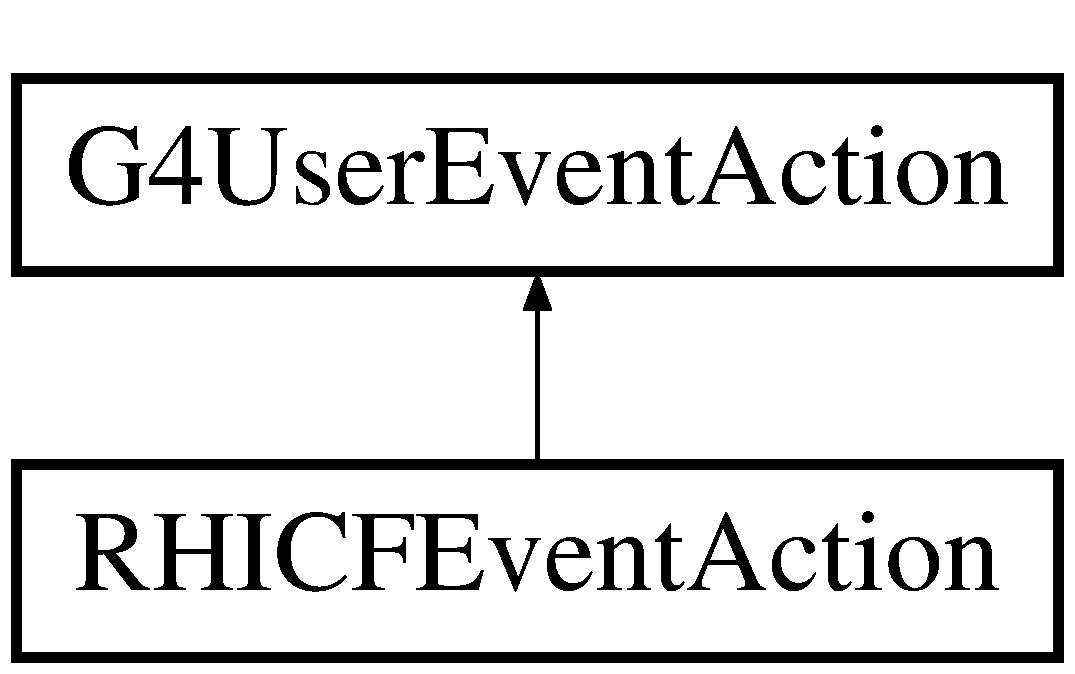
\includegraphics[height=2.000000cm]{class_r_h_i_c_f_event_action}
\end{center}
\end{figure}
\subsection*{Public Member Functions}
\begin{DoxyCompactItemize}
\item 
\hypertarget{class_r_h_i_c_f_event_action_a92b97430fa42224e11e4544fe4904a31}{}{\bfseries R\+H\+I\+C\+F\+Event\+Action} (\hyperlink{class_b5_primary_generator_action}{B5\+Primary\+Generator\+Action} $\ast$)\label{class_r_h_i_c_f_event_action_a92b97430fa42224e11e4544fe4904a31}

\item 
\hypertarget{class_r_h_i_c_f_event_action_a18d53bb5e543926414fa188bafc21100}{}virtual void {\bfseries Begin\+Of\+Event\+Action} (const G4\+Event $\ast$)\label{class_r_h_i_c_f_event_action_a18d53bb5e543926414fa188bafc21100}

\item 
\hypertarget{class_r_h_i_c_f_event_action_aacf0480914ecf3223d6d65891f598a69}{}virtual void {\bfseries End\+Of\+Event\+Action} (const G4\+Event $\ast$)\label{class_r_h_i_c_f_event_action_aacf0480914ecf3223d6d65891f598a69}

\end{DoxyCompactItemize}


The documentation for this class was generated from the following files\+:\begin{DoxyCompactItemize}
\item 
R\+H\+I\+C\+F\+Event\+Action.\+hh\item 
R\+H\+I\+C\+F\+Event\+Action.\+cc\end{DoxyCompactItemize}

\hypertarget{class_r_h_i_c_f_extra_physics}{}\section{R\+H\+I\+C\+F\+Extra\+Physics Class Reference}
\label{class_r_h_i_c_f_extra_physics}\index{R\+H\+I\+C\+F\+Extra\+Physics@{R\+H\+I\+C\+F\+Extra\+Physics}}
Inheritance diagram for R\+H\+I\+C\+F\+Extra\+Physics\+:\begin{figure}[H]
\begin{center}
\leavevmode
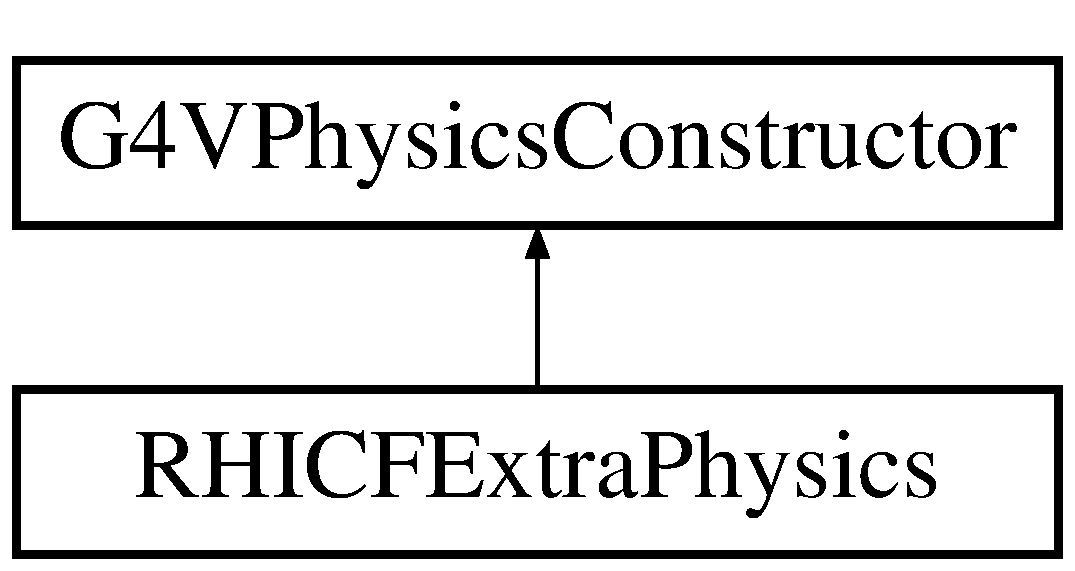
\includegraphics[height=2.000000cm]{class_r_h_i_c_f_extra_physics}
\end{center}
\end{figure}
\subsection*{Public Member Functions}
\begin{DoxyCompactItemize}
\item 
\hypertarget{class_r_h_i_c_f_extra_physics_aed1fbbadeeaa965b447e0f452d093e66}{}virtual void {\bfseries Construct\+Particle} ()\label{class_r_h_i_c_f_extra_physics_aed1fbbadeeaa965b447e0f452d093e66}

\item 
\hypertarget{class_r_h_i_c_f_extra_physics_af5ec71a267db3f26879f1773c5d512b4}{}virtual void {\bfseries Construct\+Process} ()\label{class_r_h_i_c_f_extra_physics_af5ec71a267db3f26879f1773c5d512b4}

\end{DoxyCompactItemize}


The documentation for this class was generated from the following files\+:\begin{DoxyCompactItemize}
\item 
R\+H\+I\+C\+F\+Extra\+Physics.\+hh\item 
R\+H\+I\+C\+F\+Extra\+Physics.\+cc\end{DoxyCompactItemize}

\hypertarget{class_r_h_i_c_f_materials}{}\section{R\+H\+I\+C\+F\+Materials Class Reference}
\label{class_r_h_i_c_f_materials}\index{R\+H\+I\+C\+F\+Materials@{R\+H\+I\+C\+F\+Materials}}
\subsection*{Public Member Functions}
\begin{DoxyCompactItemize}
\item 
\hypertarget{class_r_h_i_c_f_materials_acd28f3e73d2a00df6d8f0ced12ec4ef2}{}G4\+Material $\ast$ {\bfseries Get\+Material} (const G4\+String)\label{class_r_h_i_c_f_materials_acd28f3e73d2a00df6d8f0ced12ec4ef2}

\end{DoxyCompactItemize}
\subsection*{Static Public Member Functions}
\begin{DoxyCompactItemize}
\item 
\hypertarget{class_r_h_i_c_f_materials_abfd60afadb7808fe5f8cf6ea64a7fd85}{}static \hyperlink{class_r_h_i_c_f_materials}{R\+H\+I\+C\+F\+Materials} $\ast$ {\bfseries Get\+Instance} ()\label{class_r_h_i_c_f_materials_abfd60afadb7808fe5f8cf6ea64a7fd85}

\end{DoxyCompactItemize}


The documentation for this class was generated from the following files\+:\begin{DoxyCompactItemize}
\item 
R\+H\+I\+C\+F\+Materials.\+hh\item 
R\+H\+I\+C\+F\+Materials.\+cc\end{DoxyCompactItemize}

\hypertarget{class_r_h_i_c_f_optical_physics}{}\section{R\+H\+I\+C\+F\+Optical\+Physics Class Reference}
\label{class_r_h_i_c_f_optical_physics}\index{R\+H\+I\+C\+F\+Optical\+Physics@{R\+H\+I\+C\+F\+Optical\+Physics}}
Inheritance diagram for R\+H\+I\+C\+F\+Optical\+Physics\+:\begin{figure}[H]
\begin{center}
\leavevmode
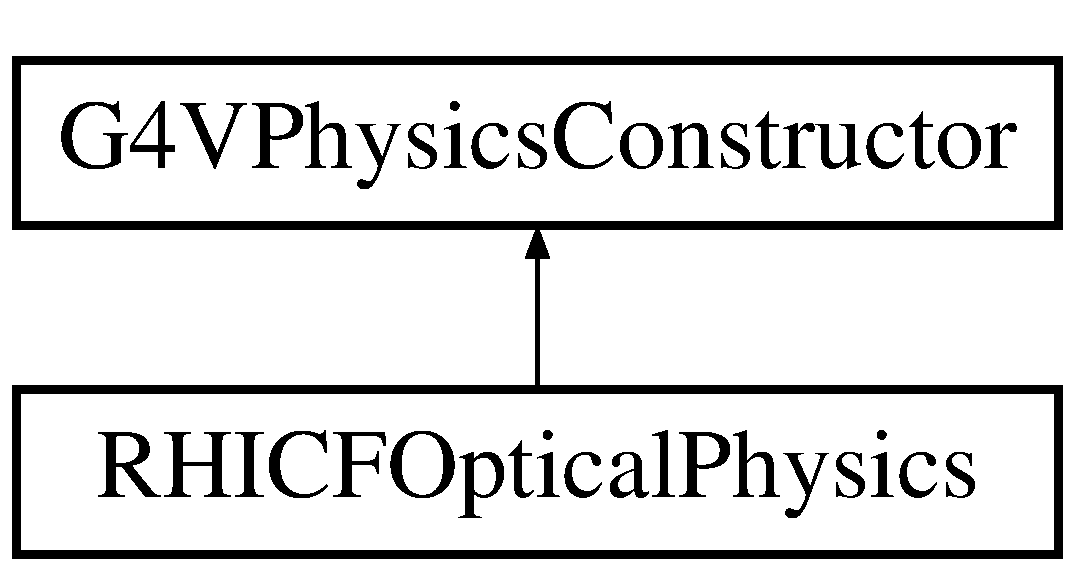
\includegraphics[height=2.000000cm]{class_r_h_i_c_f_optical_physics}
\end{center}
\end{figure}
\subsection*{Public Member Functions}
\begin{DoxyCompactItemize}
\item 
\hypertarget{class_r_h_i_c_f_optical_physics_a4e4d3f7d099e55bee93c1d0bdae100f2}{}{\bfseries R\+H\+I\+C\+F\+Optical\+Physics} (G4bool toggle=true)\label{class_r_h_i_c_f_optical_physics_a4e4d3f7d099e55bee93c1d0bdae100f2}

\item 
\hypertarget{class_r_h_i_c_f_optical_physics_adf633ad46bfadaf066b1d6aa32f422ee}{}virtual void {\bfseries Construct\+Particle} ()\label{class_r_h_i_c_f_optical_physics_adf633ad46bfadaf066b1d6aa32f422ee}

\item 
\hypertarget{class_r_h_i_c_f_optical_physics_a0ee71df377c8ba3b044bc837562934c6}{}virtual void {\bfseries Construct\+Process} ()\label{class_r_h_i_c_f_optical_physics_a0ee71df377c8ba3b044bc837562934c6}

\item 
\hypertarget{class_r_h_i_c_f_optical_physics_aa4427e0bee465f18b892fdd25004eee1}{}G4\+Op\+W\+L\+S $\ast$ {\bfseries Get\+R\+H\+I\+C\+F\+Process} ()\label{class_r_h_i_c_f_optical_physics_aa4427e0bee465f18b892fdd25004eee1}

\item 
\hypertarget{class_r_h_i_c_f_optical_physics_adfd9cd4490bf681b51e5ccd3864a80db}{}G4\+Cerenkov $\ast$ {\bfseries Get\+Cerenkov\+Process} ()\label{class_r_h_i_c_f_optical_physics_adfd9cd4490bf681b51e5ccd3864a80db}

\item 
\hypertarget{class_r_h_i_c_f_optical_physics_a4d3e5ed27a61fcd814cf791739d7ad51}{}G4\+Scintillation $\ast$ {\bfseries Get\+Scintillation\+Process} ()\label{class_r_h_i_c_f_optical_physics_a4d3e5ed27a61fcd814cf791739d7ad51}

\item 
\hypertarget{class_r_h_i_c_f_optical_physics_aad6f5d100c840c6cf85615c8e29a8973}{}G4\+Op\+Absorption $\ast$ {\bfseries Get\+Absorption\+Process} ()\label{class_r_h_i_c_f_optical_physics_aad6f5d100c840c6cf85615c8e29a8973}

\item 
\hypertarget{class_r_h_i_c_f_optical_physics_abdc3735a932b50ddcc8e071cde091e11}{}G4\+Op\+Rayleigh $\ast$ {\bfseries Get\+Rayleigh\+Scattering\+Process} ()\label{class_r_h_i_c_f_optical_physics_abdc3735a932b50ddcc8e071cde091e11}

\item 
\hypertarget{class_r_h_i_c_f_optical_physics_ac23aac998b7b4460a8d4da6aae7ae32d}{}G4\+Op\+Mie\+H\+G $\ast$ {\bfseries Get\+Mie\+H\+G\+Scattering\+Process} ()\label{class_r_h_i_c_f_optical_physics_ac23aac998b7b4460a8d4da6aae7ae32d}

\item 
\hypertarget{class_r_h_i_c_f_optical_physics_a50c493d6ed4ddf5e5ef4282932f18542}{}G4\+Op\+Boundary\+Process $\ast$ {\bfseries Get\+Boundary\+Process} ()\label{class_r_h_i_c_f_optical_physics_a50c493d6ed4ddf5e5ef4282932f18542}

\item 
\hypertarget{class_r_h_i_c_f_optical_physics_a75bcc20717f634aba7bc760c938e91c9}{}void {\bfseries Set\+Nb\+Of\+Photons\+Cerenkov} (G4int)\label{class_r_h_i_c_f_optical_physics_a75bcc20717f634aba7bc760c938e91c9}

\end{DoxyCompactItemize}


The documentation for this class was generated from the following files\+:\begin{DoxyCompactItemize}
\item 
R\+H\+I\+C\+F\+Optical\+Physics.\+hh\item 
R\+H\+I\+C\+F\+Optical\+Physics.\+cc\end{DoxyCompactItemize}

\hypertarget{class_r_h_i_c_f_physics_list}{}\section{R\+H\+I\+C\+F\+Physics\+List Class Reference}
\label{class_r_h_i_c_f_physics_list}\index{R\+H\+I\+C\+F\+Physics\+List@{R\+H\+I\+C\+F\+Physics\+List}}
Inheritance diagram for R\+H\+I\+C\+F\+Physics\+List\+:\begin{figure}[H]
\begin{center}
\leavevmode
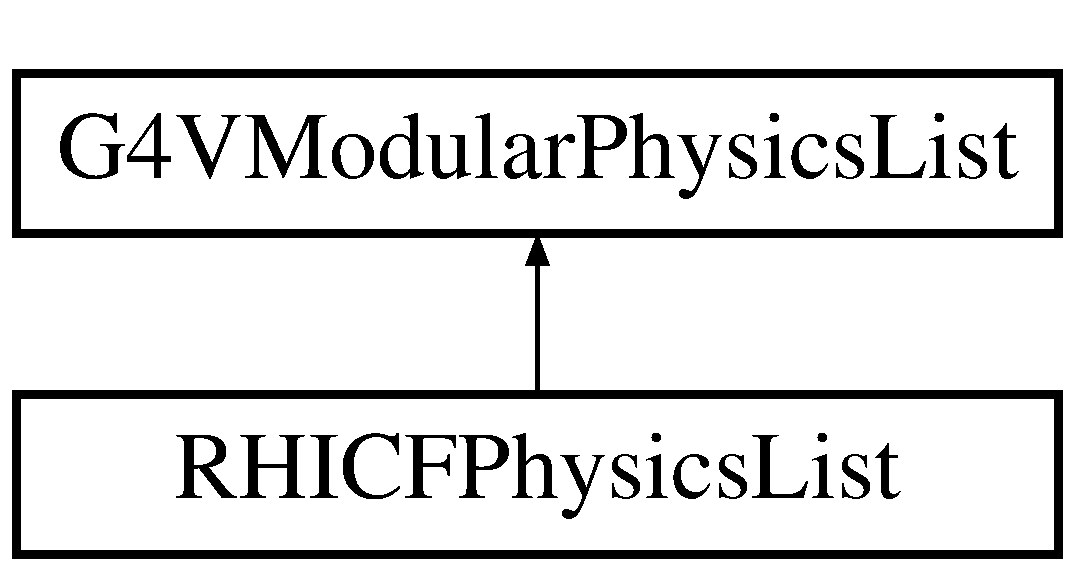
\includegraphics[height=2.000000cm]{class_r_h_i_c_f_physics_list}
\end{center}
\end{figure}
\subsection*{Public Member Functions}
\begin{DoxyCompactItemize}
\item 
\hypertarget{class_r_h_i_c_f_physics_list_a5e4bf3ac92e1ea73dbcdbf0c74a60487}{}{\bfseries R\+H\+I\+C\+F\+Physics\+List} (G4\+String)\label{class_r_h_i_c_f_physics_list_a5e4bf3ac92e1ea73dbcdbf0c74a60487}

\item 
\hypertarget{class_r_h_i_c_f_physics_list_ae98a93d472ac75f6d984dde9d91b7575}{}void {\bfseries Set\+Cuts} ()\label{class_r_h_i_c_f_physics_list_ae98a93d472ac75f6d984dde9d91b7575}

\item 
\hypertarget{class_r_h_i_c_f_physics_list_a2e64cb1fbb790eb0efd3b6f1a5dad787}{}void {\bfseries Set\+Cut\+For\+Gamma} (G4double)\label{class_r_h_i_c_f_physics_list_a2e64cb1fbb790eb0efd3b6f1a5dad787}

\item 
\hypertarget{class_r_h_i_c_f_physics_list_a1959042d3c6d12e6251209f25ffd3118}{}void {\bfseries Set\+Cut\+For\+Electron} (G4double)\label{class_r_h_i_c_f_physics_list_a1959042d3c6d12e6251209f25ffd3118}

\item 
\hypertarget{class_r_h_i_c_f_physics_list_ade29c53c57444dd9085b0055f1848f3e}{}void {\bfseries Set\+Cut\+For\+Positron} (G4double)\label{class_r_h_i_c_f_physics_list_ade29c53c57444dd9085b0055f1848f3e}

\item 
\hypertarget{class_r_h_i_c_f_physics_list_af39cf17eace11546d98872f25e4ce120}{}void {\bfseries Set\+Step\+Max} (G4double)\label{class_r_h_i_c_f_physics_list_af39cf17eace11546d98872f25e4ce120}

\item 
\hypertarget{class_r_h_i_c_f_physics_list_a18f4a0f48e0d35fc2eda861ca8d2380e}{}\hyperlink{class_r_h_i_c_f_step_max}{R\+H\+I\+C\+F\+Step\+Max} $\ast$ {\bfseries Get\+Step\+Max\+Process} ()\label{class_r_h_i_c_f_physics_list_a18f4a0f48e0d35fc2eda861ca8d2380e}

\item 
\hypertarget{class_r_h_i_c_f_physics_list_aba078afb485583c65dd3fb6adb154b84}{}void {\bfseries Add\+Step\+Max} ()\label{class_r_h_i_c_f_physics_list_aba078afb485583c65dd3fb6adb154b84}

\item 
\hypertarget{class_r_h_i_c_f_physics_list_a51ce859d9bc4ea6d9e6a968ccf19c0cc}{}void \hyperlink{class_r_h_i_c_f_physics_list_a51ce859d9bc4ea6d9e6a968ccf19c0cc}{Remove\+From\+Physics\+List} (const G4\+String \&)\label{class_r_h_i_c_f_physics_list_a51ce859d9bc4ea6d9e6a968ccf19c0cc}

\begin{DoxyCompactList}\small\item\em Remove specific physics from physics list. \end{DoxyCompactList}\item 
\hypertarget{class_r_h_i_c_f_physics_list_a77338f7345ed2c30ff30be204f4a37af}{}void \hyperlink{class_r_h_i_c_f_physics_list_a77338f7345ed2c30ff30be204f4a37af}{Clear\+Physics} ()\label{class_r_h_i_c_f_physics_list_a77338f7345ed2c30ff30be204f4a37af}

\begin{DoxyCompactList}\small\item\em Make sure that the physics list is empty. \end{DoxyCompactList}\item 
\hypertarget{class_r_h_i_c_f_physics_list_a5f70eec45caa590e719662ad76a98e8d}{}virtual void {\bfseries Construct\+Particle} ()\label{class_r_h_i_c_f_physics_list_a5f70eec45caa590e719662ad76a98e8d}

\item 
\hypertarget{class_r_h_i_c_f_physics_list_afc31964033ef0983b18bd2f34e13a6fb}{}virtual void {\bfseries Construct\+Process} ()\label{class_r_h_i_c_f_physics_list_afc31964033ef0983b18bd2f34e13a6fb}

\item 
\hypertarget{class_r_h_i_c_f_physics_list_a0960421ee6094d55494ca654af3beff4}{}void {\bfseries Set\+Absorption} (G4bool)\label{class_r_h_i_c_f_physics_list_a0960421ee6094d55494ca654af3beff4}

\item 
\hypertarget{class_r_h_i_c_f_physics_list_a25c8f0671b5c23a38d7a87a3fe018684}{}void {\bfseries Set\+Nb\+Of\+Photons\+Cerenkov} (G4int)\label{class_r_h_i_c_f_physics_list_a25c8f0671b5c23a38d7a87a3fe018684}

\item 
\hypertarget{class_r_h_i_c_f_physics_list_aed774051f4d69c451c9f332a55315f00}{}void {\bfseries Set\+Verbose} (G4int)\label{class_r_h_i_c_f_physics_list_aed774051f4d69c451c9f332a55315f00}

\end{DoxyCompactItemize}


The documentation for this class was generated from the following files\+:\begin{DoxyCompactItemize}
\item 
R\+H\+I\+C\+F\+Physics\+List.\+hh\item 
R\+H\+I\+C\+F\+Physics\+List.\+cc\end{DoxyCompactItemize}

\hypertarget{class_r_h_i_c_f_physics_list_messenger}{}\section{R\+H\+I\+C\+F\+Physics\+List\+Messenger Class Reference}
\label{class_r_h_i_c_f_physics_list_messenger}\index{R\+H\+I\+C\+F\+Physics\+List\+Messenger@{R\+H\+I\+C\+F\+Physics\+List\+Messenger}}


Provide control of the physics list and cut parameters.  




{\ttfamily \#include $<$R\+H\+I\+C\+F\+Physics\+List\+Messenger.\+hh$>$}

Inheritance diagram for R\+H\+I\+C\+F\+Physics\+List\+Messenger\+:\begin{figure}[H]
\begin{center}
\leavevmode
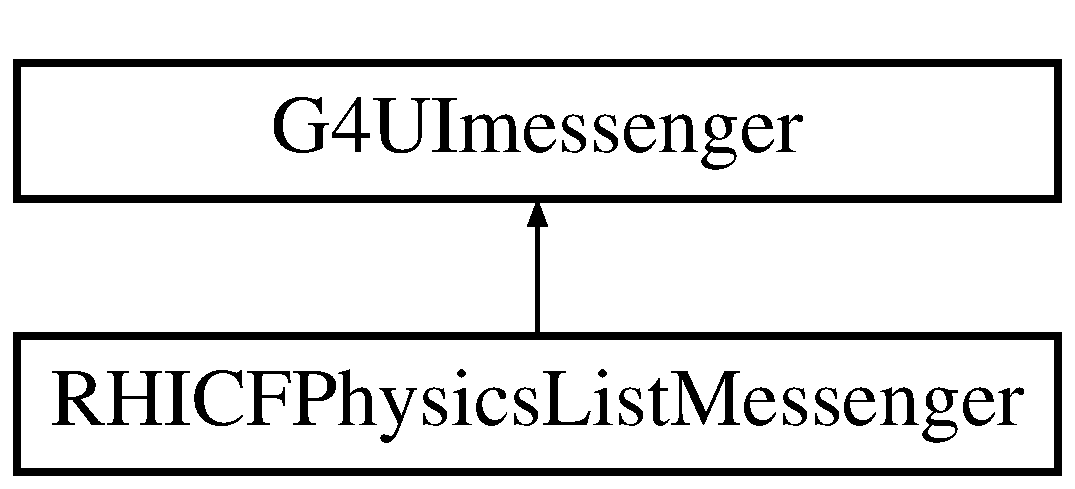
\includegraphics[height=2.000000cm]{class_r_h_i_c_f_physics_list_messenger}
\end{center}
\end{figure}
\subsection*{Public Member Functions}
\begin{DoxyCompactItemize}
\item 
\hypertarget{class_r_h_i_c_f_physics_list_messenger_ad5e2d9fc22274c779ac1dac28bd5eece}{}{\bfseries R\+H\+I\+C\+F\+Physics\+List\+Messenger} (\hyperlink{class_r_h_i_c_f_physics_list}{R\+H\+I\+C\+F\+Physics\+List} $\ast$)\label{class_r_h_i_c_f_physics_list_messenger_ad5e2d9fc22274c779ac1dac28bd5eece}

\item 
\hypertarget{class_r_h_i_c_f_physics_list_messenger_ac4d12b8f3f3b71ff30ee36e2bacf369c}{}virtual void {\bfseries Set\+New\+Value} (G4\+U\+Icommand $\ast$, G4\+String)\label{class_r_h_i_c_f_physics_list_messenger_ac4d12b8f3f3b71ff30ee36e2bacf369c}

\end{DoxyCompactItemize}


\subsection{Detailed Description}
Provide control of the physics list and cut parameters. 

The documentation for this class was generated from the following files\+:\begin{DoxyCompactItemize}
\item 
R\+H\+I\+C\+F\+Physics\+List\+Messenger.\+hh\item 
R\+H\+I\+C\+F\+Physics\+List\+Messenger.\+cc\end{DoxyCompactItemize}

\hypertarget{class_r_h_i_c_f_run_action}{}\section{R\+H\+I\+C\+F\+Run\+Action Class Reference}
\label{class_r_h_i_c_f_run_action}\index{R\+H\+I\+C\+F\+Run\+Action@{R\+H\+I\+C\+F\+Run\+Action}}


Run action class.  




{\ttfamily \#include $<$R\+H\+I\+C\+F\+Run\+Action.\+hh$>$}

Inheritance diagram for R\+H\+I\+C\+F\+Run\+Action\+:\begin{figure}[H]
\begin{center}
\leavevmode
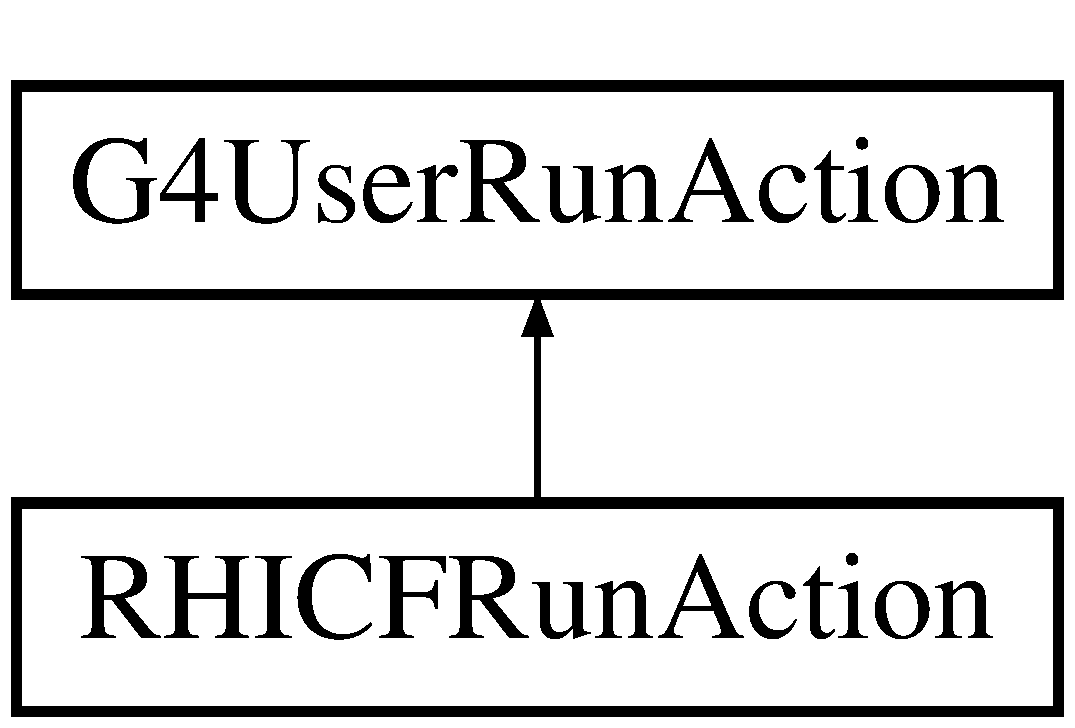
\includegraphics[height=2.000000cm]{class_r_h_i_c_f_run_action}
\end{center}
\end{figure}
\subsection*{Public Member Functions}
\begin{DoxyCompactItemize}
\item 
\hypertarget{class_r_h_i_c_f_run_action_a9c136cf2ae3718305e337f9f1d27bbd2}{}virtual void {\bfseries Begin\+Of\+Run\+Action} (const G4\+Run $\ast$)\label{class_r_h_i_c_f_run_action_a9c136cf2ae3718305e337f9f1d27bbd2}

\item 
\hypertarget{class_r_h_i_c_f_run_action_ab3f9bbac27bac8af0f8f4dfada553a30}{}virtual void {\bfseries End\+Of\+Run\+Action} (const G4\+Run $\ast$)\label{class_r_h_i_c_f_run_action_ab3f9bbac27bac8af0f8f4dfada553a30}

\end{DoxyCompactItemize}


\subsection{Detailed Description}
Run action class. 

The documentation for this class was generated from the following files\+:\begin{DoxyCompactItemize}
\item 
R\+H\+I\+C\+F\+Run\+Action.\+hh\item 
R\+H\+I\+C\+F\+Run\+Action.\+cc\end{DoxyCompactItemize}

\hypertarget{class_r_h_i_c_f_step_max}{}\section{R\+H\+I\+C\+F\+Step\+Max Class Reference}
\label{class_r_h_i_c_f_step_max}\index{R\+H\+I\+C\+F\+Step\+Max@{R\+H\+I\+C\+F\+Step\+Max}}
Inheritance diagram for R\+H\+I\+C\+F\+Step\+Max\+:\begin{figure}[H]
\begin{center}
\leavevmode
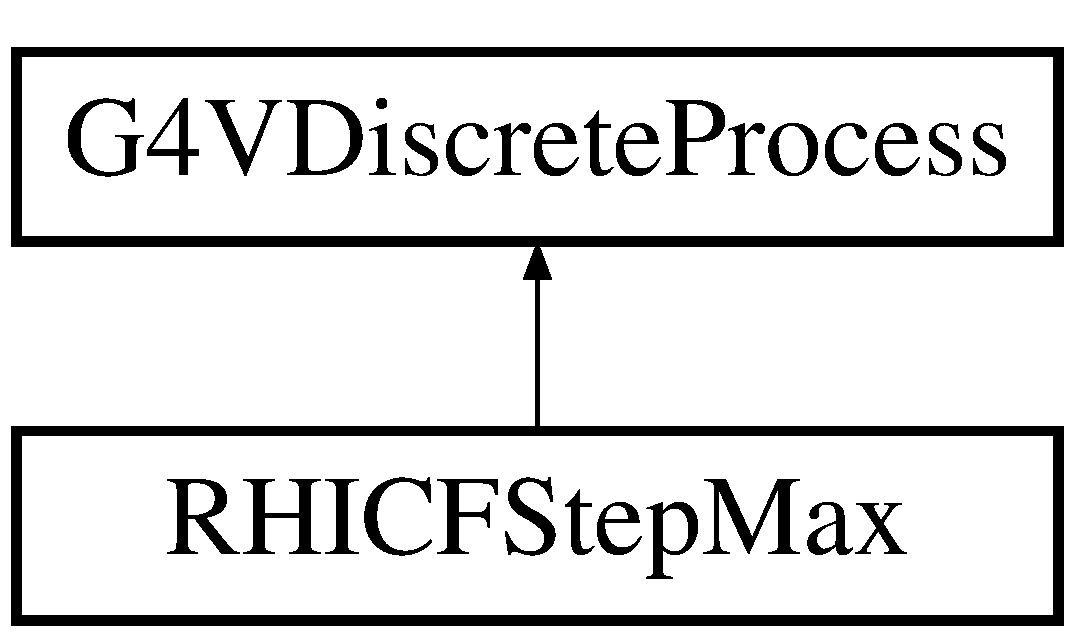
\includegraphics[height=2.000000cm]{class_r_h_i_c_f_step_max}
\end{center}
\end{figure}
\subsection*{Public Member Functions}
\begin{DoxyCompactItemize}
\item 
\hypertarget{class_r_h_i_c_f_step_max_aae289bfe6b0e528eec5fd7f76cdd17d4}{}{\bfseries R\+H\+I\+C\+F\+Step\+Max} (const G4\+String \&process\+Name=\char`\"{}User\+Step\+Max\char`\"{})\label{class_r_h_i_c_f_step_max_aae289bfe6b0e528eec5fd7f76cdd17d4}

\item 
\hypertarget{class_r_h_i_c_f_step_max_a30514c9ca58f851c078206f3f45ae345}{}{\bfseries R\+H\+I\+C\+F\+Step\+Max} (\hyperlink{class_r_h_i_c_f_step_max}{R\+H\+I\+C\+F\+Step\+Max} \&)\label{class_r_h_i_c_f_step_max_a30514c9ca58f851c078206f3f45ae345}

\item 
\hypertarget{class_r_h_i_c_f_step_max_ac3278c1ddb1cf246f1179e0e5b473f4c}{}virtual G4bool {\bfseries Is\+Applicable} (const G4\+Particle\+Definition \&)\label{class_r_h_i_c_f_step_max_ac3278c1ddb1cf246f1179e0e5b473f4c}

\item 
\hypertarget{class_r_h_i_c_f_step_max_a2aa60672d93c58b7ae2030886ff8d49e}{}void {\bfseries Set\+Step\+Max} (G4double)\label{class_r_h_i_c_f_step_max_a2aa60672d93c58b7ae2030886ff8d49e}

\item 
\hypertarget{class_r_h_i_c_f_step_max_a46240c85112d681e3e53a1c56712439c}{}G4double {\bfseries Get\+Step\+Max} ()\label{class_r_h_i_c_f_step_max_a46240c85112d681e3e53a1c56712439c}

\item 
\hypertarget{class_r_h_i_c_f_step_max_aeae09e23a80e849d445df310933f0579}{}virtual G4double {\bfseries Post\+Step\+Get\+Physical\+Interaction\+Length} (const G4\+Track \&track, G4double previous\+Step\+Size, G4\+Force\+Condition $\ast$condition)\label{class_r_h_i_c_f_step_max_aeae09e23a80e849d445df310933f0579}

\item 
\hypertarget{class_r_h_i_c_f_step_max_ae59e251e8ef437c3752c2fa968d0084d}{}virtual G4\+V\+Particle\+Change $\ast$ {\bfseries Post\+Step\+Do\+It} (const G4\+Track \&, const G4\+Step \&)\label{class_r_h_i_c_f_step_max_ae59e251e8ef437c3752c2fa968d0084d}

\end{DoxyCompactItemize}
\subsection*{Protected Member Functions}
\begin{DoxyCompactItemize}
\item 
\hypertarget{class_r_h_i_c_f_step_max_a82145133afd99cda8d5f1de9e1c53c64}{}G4double {\bfseries Get\+Mean\+Free\+Path} (const G4\+Track \&, G4double, G4\+Force\+Condition $\ast$)\label{class_r_h_i_c_f_step_max_a82145133afd99cda8d5f1de9e1c53c64}

\end{DoxyCompactItemize}


The documentation for this class was generated from the following files\+:\begin{DoxyCompactItemize}
\item 
R\+H\+I\+C\+F\+Step\+Max.\+hh\item 
R\+H\+I\+C\+F\+Step\+Max.\+cc\end{DoxyCompactItemize}

\chapter{File Documentation}
\hypertarget{_b5_primary_generator_action_8hh}{}\section{B5\+Primary\+Generator\+Action.\+hh File Reference}
\label{_b5_primary_generator_action_8hh}\index{B5\+Primary\+Generator\+Action.\+hh@{B5\+Primary\+Generator\+Action.\+hh}}


Definition of the \hyperlink{class_b5_primary_generator_action}{B5\+Primary\+Generator\+Action} class.  


{\ttfamily \#include \char`\"{}G4\+V\+User\+Primary\+Generator\+Action.\+hh\char`\"{}}\\*
{\ttfamily \#include \char`\"{}globals.\+hh\char`\"{}}\\*
\subsection*{Classes}
\begin{DoxyCompactItemize}
\item 
class \hyperlink{class_b5_primary_generator_action}{B5\+Primary\+Generator\+Action}
\end{DoxyCompactItemize}


\subsection{Detailed Description}
Definition of the \hyperlink{class_b5_primary_generator_action}{B5\+Primary\+Generator\+Action} class. 


%--- End generated contents ---

% Index
\backmatter
\newpage
\phantomsection
\clearemptydoublepage
\addcontentsline{toc}{chapter}{Index}
\printindex

\end{document}
